\documentclass[11pt,a4paper]{article}

% --- Packages ---
\usepackage[utf8]{inputenc}
\usepackage[T1]{fontenc}
\usepackage{amsmath,amssymb,amsthm}
\usepackage{graphicx}
\usepackage{booktabs}
\usepackage{hyperref}
\usepackage{cleveref}
\usepackage{natbib}
\usepackage[margin=1in]{geometry}
\usepackage{xcolor}
\usepackage{algorithm}
\usepackage{algpseudocode}

% --- Theorem environments ---
\newtheorem{theorem}{Theorem}
\newtheorem{lemma}[theorem]{Lemma}
\newtheorem{proposition}[theorem]{Proposition}
\newtheorem{corollary}[theorem]{Corollary}
\newtheorem{definition}{Definition}
\newtheorem{remark}{Remark}

% --- Macros ---
% \cola{} forces upright shape so it renders correctly inside theorem/lemma/
% definition bodies (which are italic by default; T1/.../m/scit is undefined).
\newcommand{\cola}{\textup{\textsc{Cola}}}
\newcommand{\E}{\mathbb{E}}
\newcommand{\Prob}{\mathbb{P}}

% Review-flag macro for items that warrant Prof. Highley's confirmation.
% Renders inline in red so flagged items are visually scannable.
% To remove all flags before submission: redefine to \newcommand{\highley}[1]{}
\newcommand{\highley}[1]{\textcolor{red}{\textbf{[Prof.~Highley:}~#1\textbf{]}}}

% --- Title ---
\title{Incentive Compatibility of Carry-Over Lottery Allocation:\\
A Manipulation Bound and Historical Comparison of the \cola{} Family}

\author{
  Timothy Highley\thanks{La Salle University. \texttt{highley@lasalle.edu}}
  \and
  Kaushik Rajan\thanks{Independent researcher. \texttt{kaushi@alumni.ncsu.edu}}
}

\date{\today}

\begin{document}

\maketitle

\begin{abstract}
The National Basketball Association (NBA) draft lottery creates a documented incentive misalignment: teams eliminated from playoff contention can improve their expected draft position by losing additional games. \citet{munro2020notanking} prove that no mechanism based on end-of-season records alone can simultaneously reward poor performance and eliminate this incentive. Carry-Over Lottery Allocation (\cola{}) sidesteps the impossibility by replacing single-season records with multi-year playoff history as the basis for draft priority \citep{highley2026cola}. We make two contributions to the \cola{} literature. First, we derive an analytic upper bound of approximately $4.0\%$ on the worst-case probability gain from pool manipulation under empirically calibrated index distributions. The bound confirms the simulation-based estimate of \citet{highley2026cola} from the analytic side and yields a closed-form sensitivity to the underlying parameters. Second, we present the first historical backtest of the \cola{} family across 26 NBA seasons (1999--2025), comparing five variants (Simple, Simple Lottery, Classic, Countdown, and Capped \cola{}) against 776 verified draft outcomes and 55 lottery-day-attributed pre-draft trades. The analysis identifies trade handling and lottery-day attribution as the two largest sources of implementation ambiguity, and quantifies the per-series tanking exposure introduced by Capped \cola{}'s stockpile bound. Together, the results support treating \cola{} as a family of mechanisms that admit multiple adoption trajectories rather than a single design.
\end{abstract}

% --- Sections ---
\section{Introduction}
\label{sec:introduction}

% Lead: Rajan. Joint revision with Highley.
%
% Structure:
% - NBA tanking problem: misaligned incentives in the current draft lottery
% - Why the current system fails (Silver's 2026 acknowledgment)
% - Impossibility results: Munro & Banchio (2020), Coreno & Balbuzanov (2022)
% - COLA as a proposed solution family (Highley, Duncan & Volkov, 2026)
% - Contributions of this paper:
%   (1) Formal manipulation bound with conditioned estimate (~4.0%)
%   (2) First systematic cross-variant historical backtest (26 seasons, 775+ records)
% - Paper organization

The National Basketball Association's draft lottery creates a well-documented incentive misalignment: teams eliminated from playoff contention can improve their expected draft position by losing additional games. This \emph{tanking} problem has persisted through multiple reform attempts, most recently prompting NBA Commissioner Adam Silver to acknowledge ``misaligned incentives'' at the 2026 All-Star Weekend press conference~\citep{silver2026allstar}.

The problem is not merely practical---it is theoretically fundamental. \citet{munro2020notanking} prove that no draft mechanism based solely on end-of-season records can simultaneously reward poor performance and eliminate tanking incentives. Their impossibility result requires only a single pathological scenario: two eliminated teams with tied records facing each other in their final game. \citet{coreno2022axiomatic} complement this with an impossibility on the preference-manipulation side, showing that no allocation rule satisfies Respect for Priority, Envy-Free up to One Object, and Strategy-Proofness simultaneously.

Carry-Over Lottery Allocation (\cola{}) sidesteps these impossibility results by replacing single-season records with multi-year playoff track records as the basis for draft priority~\citep{highley2026cola}. Under \cola{}, a team's lottery index accumulates across seasons of missed playoffs and diminishes upon playoff success, decoupling draft odds from within-season effort. The original paper establishes incentive compatibility (IC) under five assumptions, four of which hold by construction. The fifth---that pool manipulation gains are negligible---is supported by simulation but lacks a formal bound.

This paper makes two contributions. First, we derive an analytic upper bound on the maximum probability gain achievable through pool manipulation (\cref{sec:bound}), showing it is at most ${\sim}4.0\%$ under empirically calibrated parameters and confirming that the simulation-based estimate of ${\sim}3.0\%$ is not an artifact of insufficient sampling. Second, we present the first systematic historical backtest of four \cola{} variants across 26 NBA seasons (1999--2025), providing a comparative empirical analysis that complements the original paper's synthetic simulations (\cref{sec:backtesting,sec:comparison}).

The remainder of this paper is organized as follows. \Cref{sec:background} reviews the impossibility results and prior reform proposals. \Cref{sec:cola-family} formally defines the \cola{} mechanism family and its four principal variants. \Cref{sec:bound} derives the manipulation bound. \Cref{sec:backtesting} describes the backtesting methodology. \Cref{sec:comparison} presents the cross-variant comparative analysis. \Cref{sec:discussion} discusses implications for NBA adoption and future work.

\section{Background and Related Work}
\label{sec:background}

% Lead: Rajan. Highley to review for accuracy.
%
% Structure:
% - NBA draft lottery history (coin flip -> weighted lottery -> 2019 reform)
% - Munro & Banchio impossibility (effort manipulation)
% - Coreno & Balbuzanov impossibility (preference manipulation)
% - Prior reform proposals (T-IC, uniform lottery)
% - Why multi-year memory escapes the impossibility

\subsection{The NBA Draft Lottery}
\label{sec:lottery-history}

The NBA assigns the top picks of its annual amateur draft via a lottery confined to the teams that did not reach the playoffs. The mechanism has been revised multiple times since its introduction, each revision motivated by an empirically observed tanking response \citep{nbalotteryhistory}. From 1966 to 1984 the league used a coin flip between the two worst-record conferences, paired with a reverse-order assignment for the remaining picks; the coin flip was abandoned after the 1984--85 ``Hakeem versus Jordan'' season produced public accusations that both Houston and Portland had tanked the final games to maximise their flip odds. From 1985 to 1989 the league used an unweighted envelope lottery among non-playoff teams. From 1990 to 2018 the lottery was weighted, with the worst team receiving a 25\% chance at the first pick and odds declining monotonically by record. The 2019 reform flattened the top three odds (the worst three teams now share a $14.0\%$ chance at the first pick) and extended the lottery to determine the top four picks rather than the top three, in response to the 2013--2017 Philadelphia ``Process'' \citep{nba2019lotteryreform}. Each revision narrowed but did not eliminate the underlying tanking incentive, and the 2019 flattening shifted some of the incentive from the bottom of the standings toward the lower-middle of the lottery pool.

\subsection{Impossibility Results}

\subsubsection{Effort Manipulation}

\citet{munro2020notanking} formalise the tanking problem as an impossibility. They define a \emph{No-Tanking Condition} (NTC): a mechanism satisfies NTC if no team can improve its expected outcome by losing. In particular, a team that misses the playoffs must not be able to improve its draft position by losing a game it could win. Their main result establishes that any mechanism mapping end-of-season records to draft probabilities, while giving worse teams strictly better odds, must violate NTC.

The proof constructs a minimal counterexample: two teams, both eliminated, with identical records and a final game against each other. The loser finishes with a worse record and therefore receives better draft odds. Both teams prefer to lose. Only a uniform lottery (equal odds for all non-playoff teams) satisfies NTC, but uniform odds abandon the goal of helping the weakest teams.

The authors propose an alternative mechanism, \emph{T-IC} (Truncated Incentive Compatibility), which tracks each team's conditional probability of finishing last and freezes allocations at the moment IC would first be violated. T-IC is optimal in theory but computationally expensive, opaque to fans, and limited to single-season scope. There are two additional fundamental issues with implementing T-IC. A precise calculation of when IC would first be violated requires knowledge of teams' precise valuation of reaching the playoffs versus how they value the draft. Additionally, it is possible, and arguably likely, that there are teams who have an incentive to tank starting with the first game of the season.

\subsubsection{Preference Manipulation}

\citet{coreno2022axiomatic} address a complementary manipulation vector: teams misreporting which players they prefer. They prove that no allocation rule simultaneously satisfies:
\begin{itemize}
    \item \textbf{Respect for Priority (RP):} higher-priority teams receive weakly better allocations~\citep{svensson1994allocation};
    \item \textbf{Envy-Free up to One Object (EF1):} no team envies another's allocation after removing one item~\citep{lipton2004approximately,budish2011combinatorial};
    \item \textbf{Strategy-Proofness (SP):} no team benefits from misreporting preferences.
\end{itemize}

We trace the constituent axioms to peer-reviewed sources. RP extends Svensson's ``weak fairness'' from queue allocation to draft priority \citep{svensson1994allocation}. EF1 originates with \citet{lipton2004approximately} and is adapted to the indivisible-goods assignment setting by \citet{budish2011combinatorial}. The Coreno-Balbuzanov construction combines these properties with strategy-proofness; the impossibility shows that any draft rule satisfying all three jointly produces a contradiction in the allocation table.

\highley{Whether RP and EF1 map cleanly onto \cola{} is the open question we deferred to your read. Our preliminary mapping: RP corresponds to longer droughts producing weakly better expected draft position (\cola{}'s priority ordering = ticket ranking), and EF1 corresponds to no team preferring another's outcome once one ``lucky'' lottery win is removed (the graduated diminishment schedule preserves perceived fairness in this sense). Strategy-proofness is the manipulation question Section~\ref{sec:bound} addresses. We are not certain whether the formal Coreno-Balbuzanov axioms admit this lift to a multi-season mechanism. If you would prefer this paragraph withdrawn, restructured, or replaced with a weaker observation (``Coreno-Balbuzanov is parallel work that does not cleanly apply''), please mark accordingly.}

HIGHLEY RESPONSE: I'll take a look at this one in more depth.

\subsection{Prior Reform Proposals}
\label{sec:prior-reform}

Beyond the T-IC mechanism of \citet{munro2020notanking}, three families of reform have appeared in the literature and the press. None has been adopted.

\paragraph{Uniform lottery.} Equal odds for all non-playoff teams. Trivially satisfies NTC but provides no reward for the worst teams, contradicting the league's stated goal of helping struggling franchises rebuild.

HIGHLEY NOTE: 3-2-1, which is likely to have a vote at the end of May, is essentially the uniform lottery but with an adjustment for the play-in and a punishment for the bottom 3 teams. Obviously does not help struggling teams.

\paragraph{Wheel proposals.} A pre-committed rotation of draft positions across teams \citep{highley2026solvable1}. The wheel removes the link between record and draft odds entirely, eliminating tanking incentives but also eliminating the redistribution property: a team in a deep rebuild cannot accelerate it through poor performance. Owner buy-in has been the dominant obstacle. \highley{The wheel proposal is sometimes attributed to Mike Zarren of the Boston Celtics; if you have a citation we should use, please add.}

HIGHLEY NOTE: I have also heard that. Apparently everyone knows it is Mike Zarren's concept, but I have not found an official source stating that.

\paragraph{Auction mechanisms.} Teams bid for draft positions using salary-cap space or future picks. Auction designs preserve rank-order priority but introduce significant complexity in cap accounting and the inter-temporal pricing of picks. No formal proposal has progressed beyond the literature, and none has been advanced by the league.

\cola{}~\citep{highley2026cola} represents a different escape route from the Munro-Banchio impossibility: rather than weakening the link between record and draft odds within a season, it relocates the relevant ``record'' to a multi-year playoff history. The single-season manipulation channel that drives the Munro-Banchio counterexample becomes ineffective because no single-season choice materially shifts the multi-year ticket pool.

\section{The \cola{} Mechanism Family}
\label{sec:cola-family}

% Lead: HIGHLEY (formal definitions, IC properties).
% Rajan drafted this section conservatively from Highley et al. (2026) and the
% Substack series (Parts 1-4 + Capped COLA post). Formal-mechanism content is
% flagged for Highley's confirmation; engineering/implementation specs match
% the backtester engine in docs/js/cola-engine.js.

We organize the \cola{} mechanism family in four layers: a common framework that defines a seven-dial configuration space (Section~\ref{sec:cola-common}), the six variants under consideration in this paper as configuration points (Section~\ref{sec:cola-variants}), the mapping from dial choices to the league-relevant properties of the resulting mechanism (Section~\ref{sec:dial-properties}), and the incentive-compatibility properties established by \citet{highley2026cola} together with the open assumption that motivates Section~\ref{sec:bound} (Section~\ref{sec:cola-ic}). The relationship to the Munro-Banchio impossibility (Section~\ref{sec:cola-impossibility}) closes the section.

\subsection{Common Framework}
\label{sec:cola-common}

\subsubsection{Lottery Index and Update Equation}
\label{sec:cola-index}

Every \cola{} variant maintains a per-team, integer-valued state across seasons and uses that state to determine draft priority in the current season. We refer to this state as the \emph{lottery index} and write $L_i^{(t)}$ for team $i$ at the end of season $t$.

\begin{definition}[Lottery Index]
\label{def:index}
For each team $i$ and season $t$, the lottery index $L_i^{(t)} \in \mathbb{Z}_{\geq 0}$ is determined by an initial value $L_i^{(0)}$, a per-season \emph{increment} $\Delta_i^{(t)}$ (variant-specific, depending on team performance and eligibility), and a per-season \emph{diminishment} $\rho_i^{(t)} \in [0, 1]$ that scales the index down based on playoff and draft outcomes:
\begin{equation}
\label{eq:index-update}
L_i^{(t+1)} = \left(L_i^{(t)} + \Delta_i^{(t)}\right) \cdot \left(1 - \rho_i^{(t)}\right).
\end{equation}
The \emph{pool} in season $t$ is $P^{(t)} = \sum_{i \in E^{(t)}} L_i^{(t)}$, where $E^{(t)} \subseteq \{1, \ldots, 30\}$ is the set of teams eligible for the lottery in that season.
\end{definition}

\highley{Definition~\ref{def:index} is our reading of the common pattern across the variants. The original paper \citep{highley2026cola} formalises Classic \cola{} more directly; we have generalised the update rule to cover Simple, Countdown, and Capped variants in a single equation. If you prefer to keep Definition~\ref{def:index} restricted to Classic \cola{} and let the other variants use their own update rules without a unifying equation, please mark accordingly.}

The three components of the update (the eligibility set $E^{(t)}$, the increment $\Delta_i^{(t)}$, and the diminishment $\rho_i^{(t)}$) are three of the seven dials that distinguish the variants. For a non-playoff team, the increment is positive (the team accumulates priority); for a team that wins a playoff series or a top draft pick, the diminishment is positive (the team consumes some or all of its accumulated priority). Section~\ref{sec:seven-dials} formalizes these three components together with four additional dials that complete the parameterization; Section~\ref{sec:variant-map} maps each variant onto its 7-tuple in the resulting configuration space.

\subsubsection{The Seven Dials of the \cola{} Configuration Space}
\label{sec:seven-dials}

Definition~\ref{def:index} identifies three dials that determine a variant's dynamics: the eligibility set $E^{(t)}$, the increment $\Delta_i^{(t)}$, and the diminishment $\rho_i^{(t)}$. Four additional dials, implicit in the prose definitions of Section~\ref{sec:cola-variants} but not yet formalized as design degrees of freedom, complete the configuration: how draft positions are assigned given the index vector, whether the index is bounded above, how long the index persists across seasons, and how identical indices are resolved. We promote these to first-class components of a unified configuration.

\begin{definition}[\cola{} Configuration]
\label{def:configuration}
A \cola{} \emph{configuration} is a 7-tuple $(E, \Delta, \rho, W, C, S, T)$ specifying:
\begin{enumerate}
    \item \textbf{Eligibility} $E^{(t)} \subseteq \{1, \ldots, 30\}$: a season-$t$ predicate selecting the teams that participate in the lottery (per Definition~\ref{def:index}).
    \item \textbf{Increment} $\Delta_i^{(t)} \in \mathbb{Z}_{\geq 0}$: a non-negative integer added to the index of each eligible team, determined by season-$t$ state (per Definition~\ref{def:index}).
    \item \textbf{Diminishment} $\rho_i^{(t)} \in [0, 1]$: the fraction of the index removed after team $i$'s playoff or draft outcome (per Definition~\ref{def:index}).
    \item \textbf{Lottery weighting} $W$: a rule mapping the index vector $L^{(t)}|_{E^{(t)}}$ to a distribution over assignments of teams to draft positions $\{1, 2, \ldots, |E^{(t)}|\}$. The rule may be deterministic (e.g., assign by index rank) or random (e.g., draw pick 1 with probability $L_i / P$, then draw pick 2 from the remainder).
    \item \textbf{Cap} $C \in \mathbb{Z}_{>0} \cup \{\infty\}$: an upper bound on $L_i^{(t)}$, enforced as $L_i^{(t)} \leftarrow \min(L_i^{(t)}, C)$ after each increment. $C = \infty$ denotes no explicit cap.
    \item \textbf{Carry-over scope} $S$: the temporal persistence rule, one of \emph{single-season} (recompute $L_i^{(t)}$ from season-$t$ state alone, no cross-season memory), \emph{unbounded multi-year} (accumulate without limit), \emph{bounded multi-year} (accumulate up to $C$), or \emph{reset-on-event} (clear the index when a specified event occurs).
    \item \textbf{Tiebreak} $T$: a total ordering on $E^{(t)}$ that resolves cases where $L_i^{(t)} = L_j^{(t)}$ for two or more eligible teams.
\end{enumerate}
A \cola{} \emph{variant} is a specification of all seven dials.
\end{definition}

Definition~\ref{def:index} expresses the dynamics of $L^{(t)}$ in terms of dials 1--3; dials 4--7 govern how those dynamics translate into draft positions ($W$), constrain the index's range ($C$) and temporal scope ($S$), and resolve ties ($T$). The four new dials are not novel mechanisms: each variant in \citet{highley2026cola} and the Substack series specifies a choice for each of them. Formalizing the four implicit choices as typed dials enables two operations: cross-variant comparison via a single configuration object, and dial-by-dial analysis of how each value affects each downstream property. Section~\ref{sec:variant-map} populates the configuration for each variant. Section~\ref{sec:dial-properties} maps the dials to four downstream league-relevant properties: incentive compatibility, manipulation gain, per-series cost, and transparency.

\highley{Dials 4--7 are new to this paper; the prose specifications of the variants in the original paper and the Substack series imply each of them but do not surface them as design degrees of freedom. Please mark any that should not be a separate dial (subsumed by another component, or not a meaningful design choice). Two candidates for re-decomposition: (a) $C$ could be folded into $\Delta$ as a $\min(\cdot, C)$ wrapper, though we have kept it separate because the per-series cost in Lemma~\ref{lem:capped-series-bound} is most cleanly stated in terms of $C$; (b) $T$ is often subsumed by $W$ in variants where the lottery weighting is non-degenerate (Classic, Simple Lottery, Countdown all resolve index ties through the random draw), but we keep it explicit because the deterministic-rank variants need it.}

\subsubsection{Variant Map}
\label{sec:variant-map}

Table~\ref{tab:variant-map} populates each of the seven dials for the six variants under consideration: the five \cola{} variants and the NBA's 2026 ``3-2-1'' proposal, included as a degenerate configuration (Section~\ref{sec:cola-tank321}). Each row is a dial; each column is a variant. Cell values follow the verbatim specifications in \citet{highley2026cola}, the Substack series \citep{highley2026solvable1,highley2026solvable3,highley2026solvable5}, and Highley's reaction post on the 3-2-1 proposal \citep{highley2026threetwoone}. The audit script \texttt{scripts/audit\_dial\_taxonomy.js} cross-checks the numeric cells against the engine constants in \texttt{docs/js/cola-engine.js}.

\begin{table}[h]
\centering
\footnotesize
\setlength{\tabcolsep}{4pt}
\renewcommand{\arraystretch}{1.25}
\begin{tabular}{@{}c >{\raggedright\arraybackslash}p{0.13\linewidth} >{\raggedright\arraybackslash}p{0.13\linewidth} >{\raggedright\arraybackslash}p{0.13\linewidth} >{\raggedright\arraybackslash}p{0.13\linewidth} >{\raggedright\arraybackslash}p{0.13\linewidth} >{\raggedright\arraybackslash}p{0.13\linewidth}@{}}
\toprule
\textbf{Dial} & \textbf{Simple} & \textbf{Simple Lottery} & \textbf{Classic} & \textbf{Countdown} & \textbf{Capped} & \textbf{3-2-1} \\
\midrule
$E$ & 22 (non-playoff + R1 losers) & 22 (same) & 14 (non-playoff) & 22 (same) & exclusion pool & tiered 16 \\
$\Delta$ & drought $+1$ & drought $+1$ & $\alpha = 1{,}000$ & McCarty $d \cdot w$ & wins $w$ (play-in \& below) & none \\
$\rho$ & reset on series win & reset on series win & 5-step, two channels & reset on advancement & 6-step + 5-step, two channels & none \\
$W$ & deterministic by drought & pre-2019 odds top-14, deterministic rest & $L_i / P$ for picks 1--4, rank for 5--14 & nested-pool MC, tickets $(6,5,4,3,2)$ & $L_i / P$ for picks 1--5, rank for 6+ & tiered balls $(2/3/2/1)$ \\
$C$ & $\infty$ & $\infty$ & $\infty$ & $\infty$ & $\Max = 150$ & n/a \\
$S$ & reset-on-event & reset-on-event & unbounded multi-year & reset-on-event & bounded multi-year & single-season \\
$T$ & most wins & subsumed by $W$ & subsumed by $W$ & subsumed by $W$ & most wins (at cap) & subsumed by $W$ \\
\bottomrule
\end{tabular}
\caption{The seven dials, evaluated for each variant. Dial labels: $E$ eligibility, $\Delta$ increment, $\rho$ diminishment, $W$ lottery weighting, $C$ cap, $S$ carry-over scope, $T$ tiebreak (per Definition~\ref{def:configuration}). Cell values trace to the original paper, the Substack series, and Highley's reaction post on the NBA 3-2-1 proposal; the audit script \texttt{scripts/audit\_dial\_taxonomy.js} cross-checks numeric cells against the engine in \texttt{docs/js/cola-engine.js}.}
\label{tab:variant-map}
\end{table}

\highley{Table~\ref{tab:variant-map} compresses the prose definitions in Section~\ref{sec:cola-variants} and the Substack series into a one-page form. Each cell was cross-checked against the backtester engine before submission. Please mark any cell whose phrasing or value does not match your intended specification. Two cells most likely to surface differences in interpretation: (a) the Capped eligibility row, where the engine implements ``effective drought $\geq 2$'' (a derived predicate) while the prose definition in Definition~\ref{def:capped-cola} states the two exclusion rules; the two framings should be equivalent but the surface differs. (b) The Countdown carry-over scope, which we label \emph{reset-on-event} via the drought-reset interpretation, though the McCarty recomputation each season also admits the \emph{single-season} label. The 3-2-1 row (explicit single-season, no carry-over, no diminishment) confirms the framing in your reaction post.}

\subsection{Variant Definitions}
\label{sec:cola-variants}

\subsubsection{Simple \cola{}}

Simple \cola{} eliminates the lottery entirely. Eligibility is broad and ranking is deterministic.

\begin{definition}[Drought]
\label{def:drought}
The \emph{drought} of team $i$ at the end of season $t$ is the maximum number of consecutive seasons up to and including $t$ in which team $i$ has neither won a playoff series nor received a top-3 lottery pick.
\end{definition}

\begin{definition}[Simple \cola{}]
\label{def:simple-cola}
The eligibility set $E^{(t)}$ is the 22 teams with zero playoff series wins in season $t$ (the 14 non-playoff teams and the 8 first-round losers). Teams are ranked by drought (descending), with most regular-season wins as tiebreaker. Draft picks are assigned in this rank order with no random component. The lottery index $L_i^{(t)}$ is the drought itself; the increment $\Delta_i^{(t)}$ is $+1$ if team $i$ neither wins a playoff series nor a top-3 pick in season $t$, and the diminishment $\rho_i^{(t)} = 1$ otherwise (the drought resets).
\end{definition}

\subsubsection{Simple Lottery \cola{}}

\begin{definition}[Simple Lottery \cola{}]
\label{def:simple-lot-cola}
Simple Lottery \cola{} shares the eligibility set, drought state, and tiebreaker of Simple \cola{} (Definition~\ref{def:simple-cola}). It applies pre-2019 NBA lottery odds (25.0\% down to 0.5\% across the worst 14 teams in the prior weighted lottery) to the top 14 of the 22 eligible teams, ranked by drought. The remaining 8 teams receive picks 15--22 in deterministic rank order.
\end{definition}

\subsubsection{Classic \cola{}}

Classic \cola{} is the variant developed in detail by \citet{highley2026cola} and the variant our manipulation bound (Section~\ref{sec:bound}) directly analyses.

\begin{definition}[Classic \cola{}]
\label{def:classic-cola}
The eligibility set is the 14 non-playoff teams. Each non-playoff team receives an increment of $\alpha = 1{,}000$ tickets per season; playoff teams receive zero increment. Diminishment applies in two channels:
\begin{itemize}
    \item \textbf{Playoff diminishment.} Champion: $\rho = 1.0$ (full reset); finals losers: $\rho = 0.75$; conference-finals losers: $\rho = 0.5$; second-round losers: $\rho = 0.25$; first-round losers: $\rho = 0$.
    \item \textbf{Draft diminishment.} Pick \#1: $\rho = 1.0$; \#2: $\rho = 0.75$; \#3: $\rho = 0.5$; \#4: $\rho = 0.25$; picks $\geq 5$: $\rho = 0$.
\end{itemize}
The two channels apply sequentially within a season. The lottery for picks 1--4 is weighted by lottery index ($p_i = L_i / P$); picks 5--14 are assigned by lottery-index rank.
\end{definition}

\highley{The diminishment fractions $\{1.0, 0.75, 0.5, 0.25\}$ and the $\alpha = 1{,}000$ increment are taken from the original paper. Please confirm that the playoff and draft channels are presented as sequential rather than multiplicative within a single season; the backtester applies them sequentially (Phase~A pre-draft state, Phase~B post-draft diminishment), but the original paper's notation could also support a multiplicative composition.}

\subsubsection{Countdown \cola{}}

\begin{definition}[McCarty Number]
\label{def:mccarty}
The \emph{McCarty number} of team $i$ at the end of season $t$ is $M_i^{(t)} = d_i^{(t)} \cdot w_i^{(t)}$, where $d_i^{(t)}$ is team $i$'s drought (Definition~\ref{def:drought}) and $w_i^{(t)}$ is its regular-season wins.
\end{definition}

\begin{definition}[Countdown \cola{}]
\label{def:countdown-cola}
The eligibility set is the same 22-team pool as Simple \cola{}. Teams are ranked by McCarty number (descending), tiebroken by wins. The 22 teams are partitioned into nested 5-team \emph{elimination pools} by rank position. Draft picks are assigned bottom-up: the first draw uses pool~5 (rank positions 22, 21, 20, 19, 18), with ticket allocation $(2, 3, 4, 5, 6)$ from worst to best within the pool; the team drawn becomes the eliminated team and receives the highest draft pick currently available. Subsequent draws follow the same template, with each pool re-formed as the higher-ranked team from the previous pool joins.
\end{definition}

\highley{Countdown \cola{} is the variant whose closed-form draw probabilities require the most care; we use 10{,}000-trial Monte Carlo throughout (Section~\ref{sec:backtesting}) rather than analytic computation. Please confirm: is the bottom-up sequence and the $(2, 3, 4, 5, 6)$ ticket allocation the canonical Countdown \cola{} from \citep{highley2026solvable3}, or is there a published refinement we should use? The Substack heat map you shared in March was the empirical reference.}

\subsubsection{Capped \cola{}}

Capped \cola{} is the variant introduced by \citet{highley2026solvable5} in response to the NBA's reported reluctance to adopt a flexible lottery line. Its design stacks several mitigations of the playoff-tanking incentive: a wins-based increment that rewards within-season effort, a hard cap on the stockpile that bounds the per-series cost of advancing in the playoffs, and a graduated playoff-diminishment schedule that smooths the cliffs of Classic \cola{}.

\begin{definition}[Capped \cola{}]
\label{def:capped-cola}
The eligibility set $E^{(t)}$ in season $t$ is defined by two exclusion rules \citep{highley2026solvable5}: (i) any team that won a top-5 lottery pick in season $t-1$ is excluded, and (ii) any team that won at least one playoff series in season $t-1$ or in season $t$ is excluded. All other teams are eligible. The increment is $\Delta_i^{(t)} = w_i^{(t)}$ for any team that finishes the regular season outside the top 6 of either conference (i.e., play-in or below); other teams receive zero increment. The lottery index is clamped continuously at $\Max$ (default 150): if any update would yield $L_i^{(t)} > \Max$, set $L_i^{(t)} = \Max$. Diminishment applies in two channels:
\begin{itemize}
    \item \textbf{Playoff diminishment (six steps).} Champion: $\rho = 1.0$; runner-up: $\rho = 0.8$; conference-finals losers: $\rho = 0.6$; second-round losers: $\rho = 0.4$; first-round losers (excluding play-in winners): $\rho = 0.2$; play-in winners losing in round 1: $\rho = 0.1$; play-in losers: $\rho = 0$.
    \item \textbf{Draft diminishment (five steps).} Pick \#1: $\rho = 1.0$; \#2: $\rho = 0.8$; \#3: $\rho = 0.6$; \#4: $\rho = 0.4$; \#5: $\rho = 0.2$; picks $\geq 6$: $\rho = 0$.
\end{itemize}
The lottery for the first five picks is raffled from the eligible pool (each team's chance equals $L_i / P$); picks 6--$|E^{(t)}|$ are assigned by lottery-index rank. The tiebreaker at the cap is most regular-season wins. The lottery is held after first-round playoff outcomes are known so that exclusion rule (ii) is resolved before the draw; first-round playoff diminishment applies before the lottery, and second-round-and-later playoff diminishment applies after.
\end{definition}

The variant is paired with a strengthened Stepien Rule: a team whose stockpile sits at the cap must retain its own first-round draft pick every other year, removing the exploit in which a capped team trades away its high-priority pick and routes the diminishment to an acquiring team that did not earn it. The opt-out provision (a team may decline a specific pick to avoid that pick's diminishment, re-entering for later picks) is documented in the methodology card of the backtester but is not modelled in the historical sweep, since the question this section answers is the calibration of $\Max$ rather than the equilibrium effect of strategic opt-outs.

\highley{Two questions on this definition. First, is the increment $\Delta_i^{(t)} = w_i^{(t)}$ correctly stated as ``regular-season wins for any team finishing outside the top 6 of either conference''? The Substack one-liner uses ``every team outside the top 6 regular-season seeds gets a wins-based increment,'' which we interpret to include play-in advancers who lose in round 1. Second, the formal name has not been finalised on your side as of the most recent thread; we are using ``Capped \cola{}'' here pending your final naming decision in the Substack writeup. If you would prefer ``Bounded \cola{}'' or another label, a single search-replace across the paper is cheap.}

\subsubsection{The NBA 3-2-1 Proposal}
\label{sec:cola-tank321}

The NBA's 2026 reform proposal (``3-2-1''), slated for an owners' vote at the end of May 2026, expands the lottery to sixteen teams across four tiers and assigns ball counts of two, three, two, and one per tier respectively. The proposal has no cross-season state, no diminishment, and no analogue of a lottery index \citep{highley2026threetwoone}. We include 3-2-1 in the variant catalogue not as a member of the \cola{} family but as a degenerate configuration that locates the \cola{} family's contribution relative to it.

\begin{definition}[NBA 3-2-1 Lottery]
\label{def:tank321}
The eligibility set $E^{(t)}$ in season $t$ contains sixteen teams: the ten teams that miss the postseason entirely; the four teams holding the 9th or 10th seed in their conference (two per conference); and the two 7v8 play-in losers whose subsequent loser's-bracket game ends in elimination. Ball allocations follow four tiers: two balls each for the three teams with the worst regular-season records; three balls each for the seven non-playoff teams above the bottom three; two balls each for the four record-9 and record-10 seeds; and one ball each for the eligible 7v8 play-in losers. The headline total is 37 balls; the actual total varies by play-in outcome (in 2026, both 7v8 losers won their loser's-bracket games and made the playoffs, leaving the fourth tier empty and the total at 35 balls). All sixteen draft slots are raffled with probability proportional to ball count.
\end{definition}

In the configuration of Definition~\ref{def:configuration}: dials $\Delta$, $\rho$, and $C$ are vacuous (zero increment, zero diminishment, no cap); the carry-over scope $S$ is \emph{single-season}; the eligibility set $E$ is the tiered 16-team pool of Definition~\ref{def:tank321}; the lottery weighting $W$ is the tiered ball allocation; and the tiebreak $T$ is resolved within the random draw. The four \cola{} dials that introduce multi-year memory collapse to default values; three dials ($E$, $W$, $S$) carry the proposal's design.

The collapse is the proposal's defining structural feature, not an incidental implementation choice. The mechanism is, in \citet{highley2026threetwoone}'s framing, ``essentially the uniform lottery but with an adjustment for the play-in and a punishment for the bottom 3 teams.'' The ``punishment'' is what makes 3-2-1 compatible with the No-Tanking Condition: by assigning the worst three teams fewer balls than the middle seven, the mechanism does not satisfy the premise of the Munro-Banchio counterexample (that worse teams have strictly better odds), and sidesteps the impossibility at the cost of abandoning the rationale for differential odds in the first place. The \cola{} family takes the opposite route: instead of flattening single-season odds, it shifts the priority basis from single-season records to multi-year playoff history through dial $S$ in modes other than \emph{single-season}. This places 3-2-1 inside the Munro-Banchio family of mechanisms that operate on single-season records, the family Section~\ref{sec:cola-impossibility} describes \cola{} as escaping.

\highley{Definition~\ref{def:tank321} reproduces the proposal as documented in your reaction post and in the CBS Sports explainer. Two open items: (a) the exact tiebreaker among teams with identical ball counts is not stated in the public proposal documents we have located; the backtester engine defaults to ``wins ASC'' (worst record breaks ties) for visual ordering, but the actual NBA tiebreaker mechanism may be more elaborate. (b) The vote at the end of May 2026 may not pass, in which case the proposal is moot but the dial-space placement (a degenerate single-season configuration that does not escape the Munro-Banchio impossibility) remains useful as a comparison baseline in Section~\ref{sec:adoption}.}

\subsection{Dials as Levers on League-Relevant Properties}
\label{sec:dial-properties}

The configuration space of Definition~\ref{def:configuration} reduces a variant comparison to a tuple comparison. The comparison is informative only when each dial corresponds to a downstream property of the resulting mechanism. Four properties dominate the league-side adoption discussion: how strongly the configuration satisfies the five incentive-compatibility assumptions (Section~\ref{sec:cola-ic}); how large a worst-case manipulation gain it admits (Section~\ref{sec:bound}); how much per-playoff-series cost it imposes on a team (Section~\ref{sec:capped-bound}); and how legible the mechanism is to fans, media, owners, and league counsel. Table~\ref{tab:dial-properties} summarizes the mapping; the four subsections below trace each property to its controlling dials with reference to the variants of Section~\ref{sec:cola-variants}.

\begin{table}[h]
\centering
\footnotesize
\setlength{\tabcolsep}{4pt}
\renewcommand{\arraystretch}{1.25}
\begin{tabular}{@{}c >{\raggedright\arraybackslash}p{0.18\linewidth} >{\raggedright\arraybackslash}p{0.22\linewidth} >{\raggedright\arraybackslash}p{0.22\linewidth} >{\raggedright\arraybackslash}p{0.18\linewidth}@{}}
\toprule
\textbf{Dial} & \textbf{IC assumptions} & \textbf{Manipulation gain} & \textbf{Per-series cost} & \textbf{Transparency} \\
\midrule
$E$       & A1, A3, A4               & Sets $P$ in bound (\S\ref{sec:bound})            & Determines which series carry consequence       & High if simple, low if exclusion-rule complex \\
$\Delta$  & A1, A2                   & Marginal $\Delta$ per within-season decision     & Indirect                                          & High if flat, lower if formulaic              \\
$\rho$    & A2, A5                   & Cliff size at each round transition               & Direct: $\rho \cdot L$ per round                  & Medium                                         \\
$W$       & A3, A4                   & Spread across rank positions                       & Decouples position from index in part             & High if deterministic, low if MC               \\
$C$       & A4, A5                   & Bounds $p_{\max}$                                  & Hard ceiling at $\eta \cdot C$ (Lemma~\ref{lem:capped-series-bound}) & Medium       \\
$S$       & Munro-Banchio escape     & Drought concentration; gain over horizon         & Lifetime cost depth                                & Medium                                         \\
$T$       & A4 edge case             & Marginal                                           & n/a                                                & High if simple                                 \\
\bottomrule
\end{tabular}
\caption{Dial-to-property mapping. Dial labels: $E$ eligibility, $\Delta$ increment, $\rho$ diminishment, $W$ lottery weighting, $C$ cap, $S$ carry-over scope, $T$ tiebreak (per Definition~\ref{def:configuration}). Cell entries describe the form the dial's influence takes; the four subsections below elaborate with reference to the variants of Section~\ref{sec:cola-variants}.}
\label{tab:dial-properties}
\end{table}

\subsubsection{Dials and the Five IC Assumptions}
\label{sec:dial-ic}

The five IC assumptions of \citet{highley2026cola} (Section~\ref{sec:cola-ic}) each impose a constraint on a subset of dials.

\paragraph{A1 (playoff primacy)} requires that the playoff-vs-draft value gap exceed the maximum draft-position advantage a team can engineer through within-season effort. The dials at risk are $E$ (whether playoff-bound teams enter the lottery) and $\Delta$ (how large the in-season increment is). Classic, with $E$ excluding playoff teams and $\Delta = \alpha$ flat across non-playoff teams, satisfies A1 by separation. Capped, with $E$ extended to play-in-and-below teams, requires that the wins-based $\Delta = w$ be small relative to the playoff-revenue gap; empirically this holds across the historical seasons.

\paragraph{A2 (playoff advancement)} is a monotonicity constraint on $\rho$: deeper playoff runs must imply weakly larger diminishment. Classic's schedule $\{0, 0.25, 0.5, 0.75, 1.0\}$ and Capped's $\{0, 0.2, 0.4, 0.6, 0.8, 1.0\}$ both satisfy A2. A shape that gave R1 losers a higher $\rho$ than CF losers would violate it.

\paragraph{A3 (picks 5--14 negligible at the margin)} is a constraint on $W$ (the lottery weighting) and on the size of $E$. The constraint is meaningful only for variants where lower picks carry residual lottery uncertainty. Classic and Simple Lottery, with their weighted lotteries above and deterministic-rank assignment below, give picks 5--14 a small expected-value gap relative to picks 1--4. Simple's purely deterministic ranking and Countdown's smooth Monte Carlo distribution change the shape of the constraint; whether A3 holds for those variants in its original form is open to interpretation.

\paragraph{A4 (pool manipulation)} is the assumption that the analytic bound of Section~\ref{sec:bound} (or its empirical surrogate from simulation) keeps the worst-case gain small. The dials most determinative are $C$ (bounds $p_i$) and $E$ (sets $P$). Capped's $C = 150$ tightens the bound by orders of magnitude relative to Classic's $C = \infty$, at the cost of compressing high-drought rewards.

\paragraph{A5 (no traded-pick protections)} is a constraint on the interaction between $\rho$ and pick trades. Section~\ref{sec:trade-handling} enumerates four candidate rules; Capped's strengthened Stepien rule is the most aggressive structural fix.

\citet{highley2026cola} establishes IC formally for Classic \cola{} via the Diet \cola{} reduction. The same five-assumption framework is the natural setup for analyzing the IC properties of the other variants in Section~\ref{sec:cola-variants}, though formal proofs for each remain open.

\subsubsection{Dials and Manipulation Gain}
\label{sec:dial-gain}

The manipulation bound of Section~\ref{sec:bound} expresses the worst-case probability gain for team $i$ as $G_i \approx p_i \cdot (\Delta / P)$, where $p_i = L_i / P$ is the team's pool share and $\Delta = L_h - L_l$ is the pool shrinkage from excluding a high-index team. The bound is increasing in $p_i$ and in $\Delta / P$; the dials that bound each factor are the dials that bound the gain.

Three dials enter directly. $E$ sets $P$ as the total pool: $P = \sum_{i \in E^{(t)}} L_i^{(t)}$. A larger eligible set (22 teams under Simple-family variants) yields a larger $P$ than a smaller set (14 teams under Classic), shrinking $\Delta / P$ at fixed $\Delta$. $\Delta$ bounds the per-team increment per season; $C$ bounds the index outright. Together $\Delta$ and $C$ bound the maximum $L_i$ any team can reach, and therefore $p_{\max}$.

Two dials enter through compounding effects. $\rho$ controls how quickly an index decays after playoff success or a top pick, determining how concentrated $L_i$ becomes over time for a single team. $S$ determines how many seasons of accumulation can compound: \emph{unbounded multi-year} (Classic) allows $L_i$ to grow without limit; \emph{bounded multi-year} (Capped) caps it at $C$; \emph{reset-on-event} (Simple variants, Countdown) caps it implicitly via the drought reset rule; \emph{single-season} (3-2-1) eliminates accumulation entirely.

Capped is the cleanest analytical case. $C = 150$ bounds $p_{\max} \leq C / P$, an order of magnitude below the maxima Classic admits historically (Sacramento under Classic accumulated $L > 11{,}000$ before the 2023--24 season; the same trajectory under Capped would have reached $C$ in the second drought year). Theorem~\ref{thm:bound}'s bound shape applies to both variants, with $C$ replacing the unconstrained historical maximum for the Capped instance.

\subsubsection{Dials and Per-Series Cost}
\label{sec:dial-cost}

The per-series cost is the maximum lottery-index forfeiture a team incurs by advancing one additional round in the playoffs. The cost measures how strongly a configuration disincentivizes deep playoff runs; an unbounded per-series cost discourages investment in late-stage playoff success. Lemma~\ref{lem:capped-series-bound} bounds the per-series cost for Capped at $0.3 \cdot C$ in the worst case (a play-in R1 winner advancing to R2) and $0.2 \cdot C$ in the typical case.

$C$ is the dominant dial. Without a cap, a team that has accumulated index over many seasons forfeits a fraction of an unbounded amount. Classic's $\rho_{\text{R1}} = 0$ keeps the R1-loser case at zero cost, but deeper rounds carry costs proportional to the accumulated index, which is unbounded under $C = \infty$. Capped's $C = 150$ bounds the per-series cost to $\eta \cdot C$ where $\eta = \max \rho$ for a single transition.

$\rho$ enters as the multiplier on $C$. A diminishment shape with smaller per-step values lowers the per-series cost at the price of weakening the manipulation-gain bound. Classic's 5-step shape (max step 0.25) and Capped's 6-step shape (max step 0.2 for typical R1 advancement, 0.3 for the play-in edge case) trade off differently on this axis.

$S$ enters by setting the depth of accumulated index a team can have at the moment a per-series cost would be paid. \emph{Unbounded multi-year} (Classic) is the worst case; \emph{bounded multi-year} (Capped) caps it at $C$; \emph{reset-on-event} (Simple variants, Countdown) caps it via the drought reset; \emph{single-season} (3-2-1) eliminates the cost entirely because no index persists to forfeit.

\subsubsection{Dials and Transparency}
\label{sec:dial-transparency}

Transparency to external audiences is the league's reported objection to mechanisms that depart from the current weighted-lottery template \citep{highley2026solvable5}. The cost falls across three layers, each affecting a different audience: fans and media (the 30-second TV graphic), GMs and owners (multi-year team planning), and league counsel (collective-bargaining and rule-change procedural questions). Each dial loads onto a different layer.

$E$ is the most visible dial at the fan layer. Classic's ``14 non-playoff teams'' is the most legible eligibility rule. Capped's exclusion pool requires explaining two conditions (top-5 pick last year and series win last or this year). The 22-team Simple-family pool extends to first-round losers, requiring a clarifying clause. The 3-2-1 tiered 16-team pool introduces eligibility for some teams that won playoff series, which requires further explanation.

$W$ is the second most visible dial. Deterministic rank assignment (Simple) is most legible. Ticket-proportional lottery (Classic, Capped) requires explaining what a ticket is. Nested-pool Monte Carlo (Countdown) requires running a simulation, which is the format least compatible with a TV graphic.

$\Delta$ and $\rho$ govern the GM-and-owner layer. A multi-year rebuild requires the GM to forecast the team's lottery position several seasons out. Classic's flat $\Delta = \alpha$ and simple $\rho$ make this tractable. Capped's wins-based $\Delta$ and 6-step $\rho$ add complexity but remain forecastable. Countdown's $\Delta = d \cdot w$ multiplies two non-monotone factors, making multi-year forecasts noisier.

$S$ governs the league-counsel layer. Multi-year scopes (Classic, Capped) introduce questions that single-season scopes (3-2-1, legacy NBA) avoid: how does mid-season team relocation, ownership change, or league realignment interact with carry-over priority? Reporting requirements and ambiguity grow with $S$. The NBA's apparent preference for single-season-scope mechanisms in the 3-2-1 proposal \citep{highley2026threetwoone} is consistent with $S$ being the dial under the most external pressure.

\subsection{Incentive Compatibility}
\label{sec:cola-ic}

Incentive compatibility is a property of a specific configuration (Definition~\ref{def:configuration}), not of the \cola{} family as a whole. \citet{highley2026cola} establish incentive compatibility for Classic \cola{} under five assumptions, four of which hold by construction in the regular-season game and one of which is supported by simulation. We summarise the assumptions here, both because they motivate the bound in Section~\ref{sec:bound} and because the alternative variants in Section~\ref{sec:cola-variants} can be classified by which subset of these assumptions they rely on; Section~\ref{sec:dial-ic} maps each assumption to its controlling dials.

\begin{enumerate}
    \item \textbf{Playoff primacy.} The expected value to a team of advancing in the playoffs (revenue, championship probability, brand) exceeds the expected value of any plausible draft-pick gain. This justifies treating playoff outcomes as the dominant priority for any team that has the option to enter the playoffs.
    \item \textbf{Playoff advancement.} Within the playoffs, advancing further is preferred to losing earlier, controlling for opponent strength.
    \item \textbf{Picks 5--14 negligible at the margin.} The expected value gap between adjacent picks in the 5--14 range is small enough that no team can profit from manipulating its position among those slots through within-season effort.
    \item \textbf{Pool manipulation negligible.} A team cannot meaningfully shift its expected draft position by manipulating which other teams are in or out of the lottery pool. This is the assumption supported by simulation in \citep{highley2026cola} and the one Section~\ref{sec:bound} converts to an analytic upper bound.
    \item \textbf{No traded-pick protections.} Pick trades do not interact with diminishment in a way that creates manipulation incentives. The strengthened Stepien Rule of Capped \cola{} is one mechanism for enforcing this assumption; Section~\ref{sec:trade-handling} examines the four pick-trade rules of \citep{highley2026solvable4} empirically.
\end{enumerate}

\highley{The above is our reading of the five assumptions from the original paper. The exact wording of (1)--(5) differs across the arXiv paper, the formal-proof video, and the Substack series; we have used the cleanest formulation we could extract. If you have a canonical numbered statement from the paper or a slide deck we should mirror, please mark and we will replace with that wording. The substantive content (which assumptions hold by construction, which require empirical support) we are confident on; the precise phrasing is the part that benefits from your direct review.}

\subsection{Relationship to Prior Impossibilities}
\label{sec:cola-impossibility}

The Munro-Banchio impossibility (Section~\ref{sec:background}) applies to mechanisms that map end-of-season records to draft probabilities. The pathological scenario --- two eliminated teams, identical records, head-to-head final game --- depends on the within-season record being the sole input to the priority ordering. Multi-year memory breaks this dependency: in the same scenario under Classic \cola{}, the loser's lottery index increases by $\alpha = 1{,}000$ tickets, but the winner's index also increases by $\alpha$ (both teams missed the playoffs), so neither team's pool share changes through the loss. The single-game manipulation is converted from a unilateral improvement to a wash.

The same argument applies to Capped \cola{} once both teams are below the wins-increment eligibility threshold. The two teams' wins-based increments differ by at most one (the winner gets one more), but the cap ($\Max = 150$) can absorb that difference whenever both teams are sufficiently far from the cap, and the per-series structure of the playoff diminishment dominates the marginal-game incentive in the regions where the cap binds. Section~\ref{sec:bound} (Lemma~\ref{lem:capped-series-bound}) makes the per-series exposure explicit.

The Coreno-Balbuzanov impossibility (Section~\ref{sec:background}) is harder to map onto \cola{} cleanly. \cola{} is a priority mechanism; the Coreno-Balbuzanov axioms are properties of allocation rules. The natural mapping interprets the lottery-index ordering as the priority and the draft selection as the allocation, but whether the resulting object satisfies RP and EF1 in the formal sense, or whether the multi-year structure makes the axioms inapplicable, remains open. \highley{This paragraph is the most speculative in the section. If you would prefer to defer the Coreno-Balbuzanov mapping to the Discussion as future work (Section~\ref{sec:limitations}) rather than addressing it here, the Section~\ref{sec:limitations} paragraph already exists; we can move the content there and leave Section~\ref{sec:cola-impossibility} focused on Munro-Banchio alone.}

\section{Pool Manipulation Bound}
\label{sec:bound}

% Lead: Rajan. Code: cola/bound.py, cola/simulate.py.
% Figures: figures/gain_vs_delta.pdf, bound_sensitivity.pdf, bound_vs_sim.pdf.

The incentive compatibility of Classic \cola{} rests on five assumptions, four of which hold by construction. The fifth---\emph{pool manipulation gains are negligible}---is supported in the original paper by simulation over 1{,}000 synthetic seasons \citep{highley2026cola}. The companion formal-proof materials close the same gap with an additional behavioral assumption ($G > $ expected pool-manipulation gain, where $G$ is the value of a single regular-season win). In this section, we present a third closure: an analytic upper bound on the manipulation gain itself, conditioned on empirically calibrated structural properties of the index distribution.

\subsection{Setup and Notation}

Let $P = \sum_{i=1}^{n} L_i$ denote the total lottery pool, where $L_i$ is team $i$'s lottery index and $n$ is the number of lottery-eligible teams. Under Classic \cola{}, each non-playoff team receives $\alpha = 1{,}000$ tickets per season, and tickets carry over across seasons. A team's probability of winning the first pick is $p_i = L_i / P$.

The \emph{pool manipulation} loophole works as follows: team $i$ deliberately loses to a high-index opponent $h$ near the playoff boundary, causing $h$ to make the playoffs. Team $h$ (with index $L_h$) exits the lottery pool and is replaced by a lower-index team $\ell$ (with index $L_\ell < L_h$). The pool shrinks by $\Delta = L_h - L_\ell > 0$.

\subsection{Exact Gain Formula}

\begin{proposition}[Manipulation Gain]
\label{prop:gain}
The probability gain for team $i$ from a pool swap of size $\Delta = L_h - L_\ell$ is:
\begin{equation}
\label{eq:gain}
G_i = \frac{L_i \cdot \Delta}{P \cdot (P - \Delta)}
\end{equation}
\end{proposition}

\begin{proof}
Before manipulation, $p_i = L_i / P$. After the swap, the new pool is $P' = P - \Delta$, and $p_i' = L_i / P'$. The gain is $G_i = p_i' - p_i = L_i \left(\frac{1}{P - \Delta} - \frac{1}{P}\right) = \frac{L_i \cdot \Delta}{P(P - \Delta)}$.
\end{proof}

\begin{remark}[First-Order Approximation]
When $\Delta \ll P$ (typically $\Delta/P \approx 4\%$), the gain simplifies to:
\begin{equation}
\label{eq:approx}
G_i \approx p_i \cdot \frac{\Delta}{P}
\end{equation}
This factors the gain into two independent ratios: the manipulator's pool share ($p_i$) and the fractional pool change ($\Delta/P$). Both have structural ceilings, which we exploit below.
\end{remark}

\subsection{Conditioned Upper Bound}

We now bound $G_{\max}$ under two empirically calibrated conditions on the index distribution.

\begin{definition}[Structural Anti-Correlation]
\label{def:anticorr}
Let $T_{\max}$ denote the maximum consecutive non-playoff years for any team, and $T_{\text{boundary}}$ the maximum consecutive non-playoff years for a team near the playoff boundary (i.e., a team that could plausibly be pushed into the playoffs by a single loss). We say the index distribution exhibits \emph{structural anti-correlation} when $T_{\text{boundary}} \ll T_{\max}$: teams with the highest indices (longest droughts) are far from the playoff boundary and thus cannot be the target of pool manipulation.
\end{definition}

\begin{theorem}[Conditioned Manipulation Bound]
\label{thm:bound}
Under structural anti-correlation with parameters $T_{\max}$, $T_{\text{boundary}}$, and average index multiplier $\bar{k}$ (where $\bar{k} = \bar{L} / \alpha$), the maximum manipulation gain satisfies:
\begin{equation}
\label{eq:bound}
G_{\max} \leq \frac{T_{\max} \cdot (T_{\text{boundary}} - 1)}{(T_{\max} + n - 1) \cdot n \cdot \bar{k}}
\end{equation}
\end{theorem}

\begin{proof}
The gain is maximized when $L_i$ is maximized and $\Delta / P$ is maximized.

\textbf{Bounding $p_{\max}$:} The highest-index team has $L_{\max} = T_{\max} \cdot \alpha$. The minimum pool size occurs when one team has $T_{\max}$ years of accumulation and the remaining $n-1$ teams each have the minimum $\alpha$: $P_{\min} = T_{\max} \cdot \alpha + (n-1) \cdot \alpha = (T_{\max} + n - 1) \cdot \alpha$. Thus $p_{\max} \leq T_{\max} / (T_{\max} + n - 1)$.

\textbf{Bounding $\Delta / P$:} The team being pushed out has at most $T_{\text{boundary}} \cdot \alpha$ tickets, and the team replacing it has at least $\alpha$. So $\Delta_{\max} = (T_{\text{boundary}} - 1) \cdot \alpha$. In steady state, $P \approx n \cdot \bar{k} \cdot \alpha$. Thus $\Delta_{\max} / P \leq (T_{\text{boundary}} - 1) / (n \cdot \bar{k})$.

Combining via the approximation in \cref{eq:approx}: $G_{\max} \leq p_{\max} \cdot (\Delta_{\max}/P)$, yielding \cref{eq:bound}.
\end{proof}

\subsection{Empirical Calibration}
\label{sec:calibration}

Plugging \cref{eq:bound} requires four numerical inputs. We adopt the following values:

\begin{itemize}
    \item $T_{\max} = 10$. The maximum consecutive non-playoff stretch observed in our 26-season backtest (\cref{sec:backtesting}) is the Sacramento Kings' 16-year drought, but the longest stretch within the steady-state period (post cold start) bounds the practical extreme at approximately ten consecutive non-playoff years. \citet{highley2026cola} reports a similar observational bound (no team in the simulated history misses more than ten consecutive years).
    \item $T_{\text{boundary}} = 5$. The maximum consecutive non-playoff drought we observe for a team near the playoff boundary (i.e., a team whose record is plausibly within one game of crossing into the playoffs). This is our calibration; we have not seen a published value in \citet{highley2026cola} or the companion materials.
    \item $n = 14$. The number of lottery-eligible teams under Classic \cola{}, equal to the league's 14 non-playoff teams.
    \item $\bar{k} = 3.1$. The average index multiplier ($\bar{L} / \alpha$), calibrated from our backtest. \citet{highley2026cola} characterises the steady-state distribution by noting that an average team's drought before reset is approximately three years; our $\bar{k} = 3.1$ matches that observation.
\end{itemize}

\highley{The four parameters above were attributed to ``Highley et al.\ (2026)'' in an earlier draft. On rereading, only $\bar{k}$ has a near-direct counterpart in the original paper (the ``average drought of three'' observation); $T_{\max}$ has an observational counterpart but no defined parameter; $T_{\text{boundary}}$ has no precedent; $n = 14$ is structural. We have relabelled them as our own calibration. Please flag if any of these values should be sourced or revised.}

\begin{equation}
G_{\max} \leq \frac{10 \cdot 4}{23 \cdot 14 \cdot 3.1} \approx 4.0\%
\end{equation}

This contains the simulation-observed maximum of $3.0\%$ across 1{,}000 seasons reported in \citet{highley2026cola} with approximately $1.3\times$ headroom. Our independent 200-season Bradley-Terry simulation confirms the bound, with observed maximum gain of $1.70\%$ (\cref{fig:bound_vs_sim}).

\subsection{Sensitivity Analysis}

\Cref{fig:bound_sensitivity} shows the bound as a function of $T_{\max}$ and $T_{\text{boundary}}$. The bound is most sensitive to $T_{\text{boundary}}$: even under pessimistic assumptions ($T_{\text{boundary}} = 7$), the bound remains below $7\%$. Under realistic conditions ($T_{\text{boundary}} \leq 5$), the bound stays below $5\%$.

\begin{figure}[t]
    \centering
    \begin{minipage}{0.48\textwidth}
        \centering
        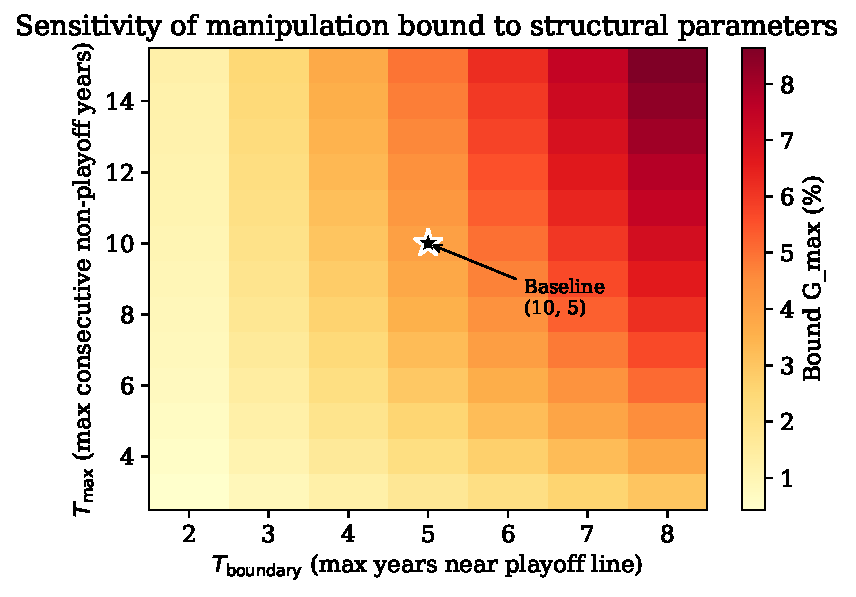
\includegraphics[width=\textwidth]{../figures/bound_sensitivity.pdf}
        \caption{Manipulation bound as a function of $T_{\max}$ and $T_{\text{boundary}}$.}
        \label{fig:bound_sensitivity}
    \end{minipage}
    \hfill
    \begin{minipage}{0.48\textwidth}
        \centering
        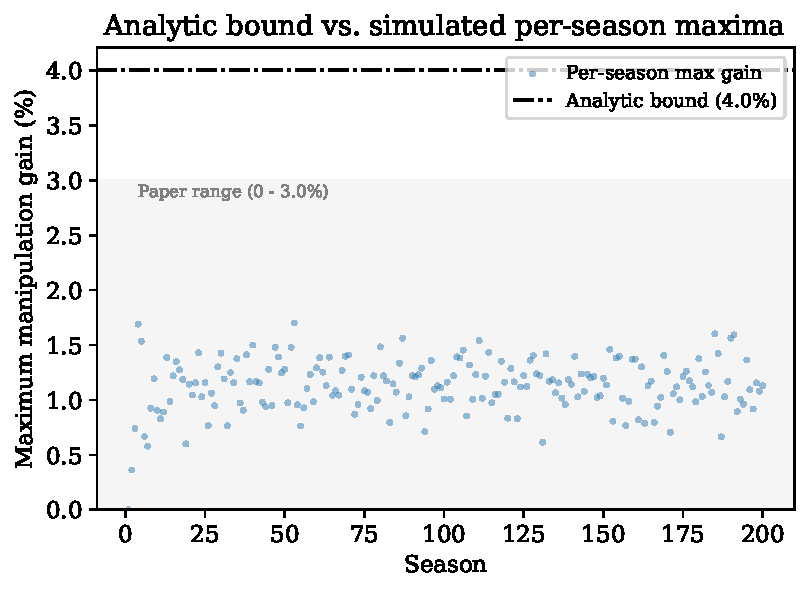
\includegraphics[width=\textwidth]{../figures/bound_vs_sim.pdf}
        \caption{Analytic bound vs.\ simulation distribution across 200 Bradley-Terry seasons.}
        \label{fig:bound_vs_sim}
    \end{minipage}
\end{figure}

\subsection{Second Source of Unboundedness}

The bound above addresses the \emph{probability} term of the manipulation incentive. However, the \emph{value} term---the pick value gap $d_k - d_{k+1}$ between adjacent draft positions---has no formal ceiling. A generational prospect could make even a small probability shift worth pursuing. Fully closing Assumption~5 would also require bounding pick value gaps, which are bounded for any realistic draft class but lack a formal argument. We leave this to future work.

\subsection{Coalitional Manipulation}

For completeness, we note that coalitional manipulation (two or more teams coordinating to shrink the pool) does not amplify individual gains. The joint gain for a coalition $\{A, B\}$ is $(L_A + L_B) \cdot \Delta / (P(P - \Delta))$. Even if two teams hold 30\% of the pool, the gain remains ${\leq}1.3\%$. Per-member gain cannot exceed the highest-index individual's gain, and coordination costs (detection risk, trust problems, sequential uncertainty) make exploitation implausible. Under McCarty \cola{}, a prisoner's dilemma arises: each conspirator prefers to defect and win the game rather than cooperate to lose.

\subsection{Per-Series Tanking Bound under Capped \cola{}}
\label{sec:capped-bound}

The Capped \cola{} variant (Definition~\ref{def:capped-cola}) was designed in part to bound the cost a team incurs by advancing in the playoffs, defusing the playoff-tanking incentive that the league flagged in conversations with \citet{highley2026solvable5}. The cap on the lottery index converts the playoff-diminishment schedule from a fraction-of-current-stockpile cost (unbounded above when the stockpile grows large) to a fraction-of-$\Max$ cost (bounded by construction). This subsection states the resulting per-series bound as a lemma.

\begin{lemma}[Per-Series Tanking Cost under Capped \cola{}]
\label{lem:capped-series-bound}
Let $\Max$ be the Capped \cola{} stockpile cap (Definition~\ref{def:capped-cola}). For any team $i$ entering the playoffs with lottery index $L_i \leq \Max$, the maximum reduction in $L_i$ attributable to winning (rather than losing) any single playoff series is bounded by:
\begin{equation}
\label{eq:capped-bound}
\Delta L_{\text{series}}^{\max} = \begin{cases}
0.3 \cdot \Max & \text{play-in advancers in round 1 (round 1 win vs.\ loss),} \\
0.2 \cdot \Max & \text{any other series advancement.}
\end{cases}
\end{equation}
At $\Max = 150$, the bound is 45 tickets for the play-in case and 30 tickets for each subsequent series.
\end{lemma}

\begin{proof}
For any single series $s$, let $\rho_{\text{lose}}$ denote the diminishment fraction applied if team $i$ loses series $s$ and $\rho_{\text{advance}}$ the diminishment if team $i$ wins $s$ and loses the immediately subsequent series. The marginal cost of advancing in $s$ is $\Delta\rho_s \cdot L_i^{\text{pre}}$, where $\Delta\rho_s = \rho_{\text{advance}} - \rho_{\text{lose}}$ and $L_i^{\text{pre}}$ is the lottery index entering series $s$.

Reading off Definition~\ref{def:capped-cola}, the per-series $\Delta\rho_s$ values are:
\begin{itemize}
    \item Play-in advancer in round 1: $\rho_{\text{lose}} = 0.1$ (play-in winners losing R1), $\rho_{\text{advance}} = 0.4$ (R2 losers), so $\Delta\rho = 0.3$.
    \item Standard round-1 advancement (non-play-in): $\rho_{\text{lose}} = 0.2$, $\rho_{\text{advance}} = 0.4$, so $\Delta\rho = 0.2$.
    \item Round 2 to conference finals: $\Delta\rho = 0.6 - 0.4 = 0.2$.
    \item Conference finals to NBA finals: $\Delta\rho = 0.8 - 0.6 = 0.2$.
    \item NBA finals to championship: $\Delta\rho = 1.0 - 0.8 = 0.2$.
\end{itemize}
The maximum is $\Delta\rho = 0.3$ in the play-in-advancer round 1 case; all other transitions yield $\Delta\rho = 0.2$. Multiplying by $L_i^{\text{pre}} \leq \Max$ (continuous cap enforcement, Definition~\ref{def:capped-cola}) yields the bounds in \eqref{eq:capped-bound}.
\end{proof}

\highley{Lemma~\ref{lem:capped-series-bound} is our restatement of the per-series claim from \citet{highley2026solvable5}. Two specific items to verify. First, the play-in transition: we have read the schedule as a single $\rho = 0.1$ tier for ``play-in winners losing in round 1'' so that the marginal cost from play-in-loser ($\rho = 0$) to play-in-winner-round-1-loser ($\rho = 0.1$) is $0.1 \cdot \Max$ and the further marginal from there to round-2-loser ($\rho = 0.4$, since play-in advancers who win round 1 then enter the standard schedule) is $0.3 \cdot \Max$. The Substack one-liner ``no playoff series win ever costs a team more than 45 lottery tickets'' is consistent with the play-in case being 45 = $0.3 \cdot 150$. If your derivation has the play-in marginal as $0.3 \cdot \Max$ at a different transition point, please flag and we will adjust. Second, our proof relies on $L_i^{\text{pre-tournament}} \leq \Max$, which follows from the continuous cap enforcement. If the cap is enforced only at end-of-regular-season (not after each diminishment event), the bound holds with the same constants but the proof requires a different argument; the Apr 19 thread settled on continuous, but flag if you would prefer the lemma stated under discrete enforcement.}

\begin{corollary}[Cumulative Run Cost]
\label{cor:capped-cumulative}
The maximum cumulative reduction in $L_i$ from a full playoff run that ends in a championship, applied to a team entering the lottery round at the cap with $L_i = \Max$, is the cap itself: $\Max$ tickets, with $L_i^{\text{post}} = 0$.
\end{corollary}

The corollary is immediate: champion diminishment is $\rho = 1.0$ (full reset), so the final state is zero regardless of starting position. Intermediate playoff exits read off Definition~\ref{def:capped-cola} directly: the cumulative reduction at each exit point equals the corresponding $\rho$ value times the entering index, capped at $\Max$. A finals-losing team at the cap therefore loses at most $0.8 \cdot \Max = 120$ tickets, a conference-finals losing team $0.6 \cdot \Max = 90$ tickets, and so on.

The per-series formulation in Lemma~\ref{lem:capped-series-bound} aligns with the public-facing framing of \citet{highley2026solvable5}, which leads with the marginal cost of each series rather than the cumulative regret across a full playoff run. The marginal framing makes the playoff-tanking incentive at the league level transparent: at $\Max = 150$, no single series win ever costs a team more than 45 lottery tickets, which is approximately a year-and-a-half of accumulation for a team near the wins-increment ceiling. Section~\ref{sec:resilience} returns to the joint resilience picture across pool manipulation (\cref{thm:bound}), per-series exposure (\cref{lem:capped-series-bound}), and multi-year strategic tanking (Section~\ref{sec:case-phi}).

\section{Backtesting Methodology}
\label{sec:backtesting}

% Lead: Rajan. Code: docs/js/cola-engine.js, docs/data/nba-data.json.

We present the first systematic historical backtest of multiple \cola{} variants using real NBA data, complementing the synthetic Bradley-Terry simulations in \citet{highley2026cola}.

\subsection{Data}

Our dataset covers 26 NBA seasons (1999--2000 through 2024--25), comprising:
\begin{itemize}
    \item 775+ team-season records from Basketball Reference, including win-loss records, playoff results (series wins/losses at each round), and draft outcomes;
    \item 776 first-round draft picks (picks 1--30, all 26 seasons);
    \item 55 pre-draft pick trades verified against lottery-day attribution (see \cref{sec:lottery-day}).
\end{itemize}

\subsection{Engine Design}

The \cola{} backtesting engine operates in two phases per season:

\begin{description}
    \item[Phase A (Pre-Draft):] Compute each team's lottery index entering the draft, based on accumulated carry-over and the current season's playoff results. This is the state displayed to users and used for draft probability calculations.
    \item[Phase B (Post-Draft):] Apply diminishment rules based on draft lottery outcomes (picks 1--4 reduce the index according to the variant's diminishment schedule). The resulting index carries forward to the next season.
\end{description}

This two-phase design resolves an off-by-one error identified by Highley in the initial implementation: without it, diminishment from the current draft would retroactively affect the probabilities used to determine that draft's outcome.

\subsubsection{Lottery-Day Attribution}
\label{sec:lottery-day}

Draft picks are frequently traded. The critical question for \cola{} index computation is: who holds the pick on \emph{lottery day} (when probabilities are determined), not on \emph{draft day} (when selections are made)?

We audited all 364 lottery picks ($14 \times 26$ seasons) and identified 8 instances where the draft-day holder differed from the lottery-day holder. The most notable: Boston held the \#1 pick on lottery day in 2017 (Philadelphia held \#3); the Fultz--Tatum swap was a post-lottery trade. Under \cola{}, Boston's index absorbs the \#1 diminishment, while Philadelphia's takes only the 50\% reduction for \#3.

\subsection{Cold Start}

\cola{} is a multi-year mechanism. Backtesting from 1999--2000 means the first several seasons have truncated drought histories. We initialize all teams with zero tickets and allow indices to build naturally. Results stabilize by approximately season 5 (2003--04). We present all 26 seasons but note the cold-start limitation.

\subsection{Variant-Specific Implementation}

\paragraph{Simple \cola{}.} 22-team eligible pool: all teams with zero playoff series wins in the current season (14 non-playoff teams + 8 first-round losers). Deterministic ordering by drought length; tiebreak by most wins.

\paragraph{Simple Lottery \cola{}.} Same drought state and 22-team pool as Simple. Pre-2019 NBA lottery odds (25.0\% down to 0.5\%) applied to the top 14 teams by drought.

\paragraph{Classic \cola{}.} Full lottery index computation per \cref{sec:cola-family}. Weighted lottery for picks 1--4; remaining picks by index rank.

\paragraph{Countdown \cola{}.} McCarty number (drought $\times$ wins) determines ranking. 5-team elimination pools with 6/5/4/3/2 tickets. Bottom-up sequential draws (21 draws total for a 22-team pool). Probabilities computed via Monte Carlo simulation per season rather than closed-form, due to the compounding effect of sequential draws. The interactive backtester runs 10{,}000 trials per season; numbers reported in case studies (Section~\ref{sec:case-mil}) come from a 100{,}000-trial reproduction with a mulberry32 PRNG seeded at 42 for paper reproducibility.

\paragraph{Capped \cola{}.} Engine implements Definition~\ref{def:capped-cola}: wins-based increment for any team finishing outside the top 6 regular-season seeds, continuous cap at $\Max$ (default 150) applied at every update step, six-step playoff diminishment (with the play-in tier separating play-in winners from play-in losers in seasons from 2019--20 onward), five-step draft diminishment, two exclusion rules (top-5 lottery winner from the prior season; playoff series winner in either the prior season or the current season), top-five lottery raffle by stockpile share, most-wins tiebreaker at the cap. The first-round playoff diminishment applies before the lottery draw because the lottery is held after round~1 (the second exclusion rule is then resolved); second-round and later diminishment applies after. To support the play-in tier, we enriched the dataset with \texttt{playInParticipant} and \texttt{playInAdvanced} fields for the 42 team-seasons in the play-in era (2019--20 bubble, 2020--21 onward), validated against the actual play-in tournament outcomes. For seasons predating the play-in tournament, the play-in tier collapses to the standard first-round-loser tier ($\rho = 0.2$).

\subsection{Limitations}

This is a \emph{static} backtest: \cola{} rules are applied to actual historical outcomes. Under a real \cola{} regime, draft outcomes would differ, which would change future drought lengths and indices. For example, the Sacramento Kings would not maintain the highest Classic \cola{} index for 6 consecutive seasons if they received the \#1 pick early in that streak. We present results with this caveat prominently noted.

Picks 15--30 reflect original holders; draft-night trades for non-lottery picks are not corrected, as these do not affect \cola{} index computation.

The Capped \cola{} backtest does not enforce two provisions of the variant's full specification: (1) the enhanced Stepien Rule (capped teams retain their own first-round pick every other year), since the pre-draft-trade dataset already contains the trade events as historical fact and re-routing them counterfactually requires the kind of dynamic backtest described in Section~\ref{sec:limitations}; and (2) the per-pick opt-out provision (a team may decline a specific pick to avoid that pick's diminishment), since the question this backtest answers is the calibration of $\Max$ rather than the equilibrium effect of strategic opt-outs. Both provisions are documented in the methodology card of the COLA Explorer~\citep{rajan2026explorer}.

\section{Comparative Analysis}
\label{sec:comparison}

% Lead: Rajan. Code: docs/js/ (all variant engines), docs/trade-simulator.html, docs/process.html.
% Figures: generate from backtester data.

This section presents a cross-variant comparative analysis using the 26-season historical backtest, examining how each \cola{} variant ranks teams differently under identical historical data. We focus on three team-season case studies that isolate distinct properties of the mechanism family (sustained drought, circumvention via repeat tanking, and elimination-pool variance), then turn to the calibration of Capped \cola{}'s stockpile cap (Section~\ref{sec:case-cap-sweep}) and the handling of traded picks (Section~\ref{sec:trade-handling}, the largest source of implementation ambiguity identified in \citet{highley2026solvable4}).

\subsection{Case Study: Sacramento Kings (Maximum Drought)}
\label{sec:case-sac}

The Sacramento Kings accumulate the highest Classic \cola{} index in the dataset, driven by a 16-season non-playoff drought (2006--07 through 2021--22) interrupted only by a single first-round appearance in 2022--23. The Kings' Classic index reaches a peak of $11{,}250$ tickets in 2017--18 before diminishment from their \#2 pick that year partially resets the accumulation; they held the top-ranked Classic \cola{} lottery position for six consecutive seasons (2012--13 through 2017--18) and regained rank~1 in 2024--25 after the 2022--23 playoff interruption.

The three \cola{} variants reward this history through different channels:
\begin{itemize}
    \item \textbf{Classic \cola{}:} The flat $\alpha = 1{,}000$ annual increment compounds across missed-playoff seasons; the Kings' index grows monotonically until diminishment events (pick \#4 in 2021--22, pick \#2 in 2017--18) partially reset it. Ranking is driven almost entirely by accumulated carry-over.
    \item \textbf{Simple \cola{}:} Deterministic ranking by drought years places the Kings near the top of the 22-team eligible pool in most years, with win-tiebreak ordering shifting them to rank~2 in seasons where another non-playoff team has a slightly longer drought.
    \item \textbf{Countdown \cola{}:} McCarty number = drought $\times$ wins. Because the Kings typically won 25--33 games during their drought, their McCarty number is lower than the Classic \cola{} index would suggest; in 2024--25 they rank second overall (McCarty~280) behind Chicago (McCarty~390).
\end{itemize}

The Kings illustrate the core design philosophy of \cola{}: teams whose losing is \emph{organic} (genuine non-competitiveness across multiple seasons) receive the strongest reward. This is the case the mechanism is optimized for.

\subsection{Case Study: Philadelphia 76ers (Tanking Circumvention)}
\label{sec:case-phi}

The 2013--14 through 2016--17 Philadelphia 76ers (the ``Process'') represent the canonical strategic-tanking sequence in the modern NBA: four consecutive top-3 lottery outcomes (picks \#3, \#3, \#1, \#3) acquired through deliberate multi-season non-competitiveness. Under the current weighted lottery, each tanked season yielded a top-tier pick; under \cola{}, graduated diminishment makes the same sequence self-defeating.

\Cref{tab:phi-process} shows Philadelphia's Classic \cola{} trajectory under static backtest:

\begin{table}[t]
\centering
\small
\begin{tabular}{lccccc}
\toprule
Season & W--L & Real Pick & \cola{} Tickets & \cola{} Rank & Top Team (Tickets) \\
\midrule
2013--14 & 19--63 & \#3 & 2{,}750 & 8 / 14 & SAC (7{,}250) \\
2014--15 & 18--64 & \#3 & 2{,}375 & 9 / 14 & SAC (8{,}250) \\
2015--16 & 10--72 & \#1 & 2{,}188 & 10 / 14 & SAC (9{,}250) \\
2016--17 & 28--54 & \#3 & 1{,}000 & 14 / 14 & SAC (10{,}250) \\
2017--18 & 52--30 & --- & 375 & --- & SAC (11{,}250) \\
\bottomrule
\end{tabular}
\caption{Philadelphia 76ers under Classic \cola{} during ``The Process.'' Each top-3 pick triggers graduated diminishment (\#1: full reset; \#3: 50\% reduction), leaving Philadelphia dead last in lottery priority by the fourth tanking season despite a 10--72 record. The 2017--18 residual of 375 reflects a 25\% second-round playoff reduction applied to the post-draft 500 ticket balance (50\% of 1{,}000) after Philadelphia's second-round playoff appearance. Sacramento's monotonic climb in the right-hand column is the counterfactual the mechanism is designed to produce: organic non-competitiveness is rewarded cumulatively while the Process extracts diminishing returns.}
\label{tab:phi-process}
\end{table}

Two properties emerge:

\begin{enumerate}
    \item \textbf{Diminishing returns to repeat tanking.} The Classic \cola{} diminishment schedule ($\{1.0, 0.75, 0.5, 0.25\}$ fractional reductions for picks \#1--4) dominates the $\alpha = 1{,}000$ annual accumulation. A team that receives a top-3 pick in year $t$ cannot re-enter the top of the lottery in year $t+1$ through tanking alone; recovery requires several non-playoff seasons with no diminishment event.
    \item \textbf{Lottery-day attribution matters.} Philadelphia's 2017--18 index of 375 assumes Philadelphia absorbs the \#3 diminishment. Because Boston held the \#1 pick on lottery day (the Fultz--Tatum swap was post-lottery), Philadelphia is charged only for \#3, not \#1. Under draft-day attribution, Philadelphia would reset to zero, Boston would retain its full index, and the mechanism's reward structure would be inverted. \Cref{sec:lottery-day} documents the audit that established this correction for all 364 lottery picks in the dataset.
\end{enumerate}

\subsection{Case Study: Milwaukee Bucks (Elimination-Pool Variance)}
\label{sec:case-mil}

Countdown \cola{} produces probability distributions that diverge sharply from both Classic \cola{} and the status-quo weighted lottery. The Milwaukee Bucks in the 2024--25 backtest provide a compact illustration.

Milwaukee's McCarty number (drought $\times$ wins) is~144, placing them seventh overall in the 22-team Countdown pool---second in the second five-team pool, behind Memphis (also McCarty~144, tiebroken by wins) and trailing pool~1 leaders Chicago (McCarty~390), Sacramento (280), Los Angeles Clippers (200), Detroit (176), and Toronto (150). A naive reading of Milwaukee's position might anticipate a meaningful \#1-pick probability: they are in the top half of the pool, and share a McCarty number with the top-ranked team of their pool.

Monte Carlo simulation (10{,}000 trials) yields $\Prob[\text{pick } \#1 \mid \text{Milwaukee}] \approx 3.7\%$ and $\E[\text{pick} \mid \text{Milwaukee}] \approx 7.22$. For comparison, Chicago (the overall pool leader) has $\Prob[\text{pick } \#1] \approx 29.7\%$ and $\E[\text{pick}] \approx 2.52$, and Memphis (Milwaukee's pool-adjacent counterpart with the same McCarty) has $\Prob[\text{pick } \#1] \approx 5.1\%$ and $\E[\text{pick}] \approx 6.28$. Countdown \cola{} runs 21 sequential bottom-up draws across nested five-team pools, and the compounding of elimination probabilities concentrates \#1-pick mass heavily on pool-1 leaders while spreading the remainder across pool-2 teams in a pattern that amplifies the effect of intra-pool ticket differences. Analytic derivation of these probabilities requires tracking $2^{21}$ branch paths; the Monte Carlo approach (applied uniformly across all 26 seasons of the backtest) is the tractable alternative.

This case highlights a tradeoff: Countdown \cola{} satisfies Highley's ``no team falls more than 4 spots'' bounded-displacement property by design, but the same elimination structure introduces probability variance that weakens the correspondence between \cola{} index rank and expected draft position. The tradeoff is material for adoption: teams and owners evaluating the mechanism in advance cannot easily reason about expected outcomes without simulation.

\subsection{Capped \cola{} Cap Calibration}
\label{sec:case-cap-sweep}

Capped \cola{} (Definition~\ref{def:capped-cola}) is parameterised by a single tunable constant: the stockpile cap $\Max$. The cap controls the trade-off between (i) ordering resolution at the top of the lottery (a higher cap permits more separation between the highest-stockpile teams) and (ii) the per-series tanking exposure given by Lemma~\ref{lem:capped-series-bound} (a higher cap raises the maximum cost a team incurs by advancing past round~1). The empirical question is whether a value of $\Max$ exists that produces both ``no more than 3--4 teams at the cap simultaneously'' (preserves separation between teams in active rebuild) and ``per-series cost of advancing in the playoffs is small relative to a typical team's annual accumulation'' (defuses the playoff-tanking incentive the league flagged).

\Cref{tab:cap-sweep} reports the 21-stable-season aggregates from the sweep over $\Max \in \{75, 100, 125, 150, 175, 200\}$, excluding the cold-start window 2000--2004 (Section~\ref{sec:backtesting}).

\begin{table}[t]
\centering
\footnotesize
\begin{tabular}{rrrrrrr}
\toprule
$\Max$ & Teams at cap (mean / max) & Sep.\ R1--R5 (mean) & Per-series max & Per-series typical & Cum.\ regret (max) \\
\midrule
75  & 6.71 / 9 &  0.9 & 22.5 & 15 & 45.0 \\
100 & 4.33 / 8 & 11.7 & 30.0 & 20 & 53.7 \\
125 & 2.86 / 4 & 27.9 & 37.5 & 25 & 53.7 \\
\textbf{150} & \textbf{1.62 / 3} & \textbf{47.7} & \textbf{45.0} & \textbf{30} & \textbf{57.6} \\
175 & 0.95 / 2 & 65.4 & 52.5 & 35 & 67.2 \\
200 & 0.52 / 2 & 76.4 & 60.0 & 40 & 76.8 \\
\bottomrule
\end{tabular}
\caption{Sensitivity of Capped \cola{} aggregates to the cap value, computed across 21 stable seasons (2005--2025) of the 26-season backtest. Per-series ``max'' = $0.3 \cdot \Max$ (the play-in advancer round~1 case from Lemma~\ref{lem:capped-series-bound}); per-series ``typical'' = $0.2 \cdot \Max$ (any other series). Cumulative regret max is the worst empirical observation across the 21 seasons. The MAX = 150 row (bold) is the variant's published default per \citet{highley2026solvable5}.}
\label{tab:cap-sweep}
\end{table}

Three patterns emerge from the sweep:

\begin{enumerate}
    \item \textbf{Sub-100 caps over-compress the lottery.} At $\Max = 75$, more than six teams sit at the cap on average and the separation between the rank-1 and rank-5 stockpile drops to under 1 ticket. The mechanism's ordering signal is destroyed: teams with materially different long-run records are treated as interchangeable, defeating the priority-ordering property the variant inherits from the broader \cola{} family.
    \item \textbf{Caps above 175 erase the cap's purpose.} At $\Max \geq 175$, fewer than one team sits at the cap on average, meaning the cap rarely binds and the variant's per-series exposure converges to a fraction of an unbounded stockpile. The playoff-tanking-incentive argument the cap was introduced to make becomes uninformative.
    \item \textbf{$\Max = 150$ is on the frontier.} The cap-150 row produces the largest separation (47.7 tickets) compatible with the ``no more than 3--4 teams at cap'' target, while keeping the per-series max at 45 tickets (approximately a year and a half of accumulation for a team near the wins-increment ceiling). The closest alternative, $\Max = 125$, produces tighter exposure (37.5 ticket max per series) at the cost of compressing separation to 27.9 tickets and pushing the typical teams-at-cap count to 2.9. Our memo-stage recommendation was $\Max = 125$ \citep{rajan2026memo}; \citet{highley2026solvable5} selects $\Max = 150$ on the rationale that the wider separation is worth the additional 7.5 tickets of per-series exposure.
\end{enumerate}

The published $\Max = 150$ choice produces fewer than two teams at the cap in 19 of 21 stable seasons, and at most three in any single season. The cap binds primarily in the late 2010s, when accumulated wins for the league's longest-rebuilding franchises (Sacramento, Detroit, Charlotte) approach the cap simultaneously. \highley{We have read the $\Max = 150$ choice as a published default in \citet{highley2026solvable5}; the Substack post phrases it as the calibration that supports the headline ``no playoff series win ever costs a team more than 45 lottery tickets.'' If you would prefer the paper present $\Max$ as a free parameter and report results across the sweep without privileging 150, we can demote the bold row in Table~\ref{tab:cap-sweep} and reframe the section as a calibration exercise. Our recommendation is to keep 150 as the default and present 125 as the closest credible alternative, mirroring the memo.}

\subsection{Trade Handling}
\label{sec:trade-handling}

\citet{highley2026solvable4} identifies four options for handling traded picks under \cola{}:

\begin{description}
    \item[Option 1 (Exclude):] Traded picks do not affect either team's \cola{} index.
    \item[Option 2 (Original Owner):] Diminishment applies to the team that originally held the pick (i.e., the team whose record determined the lottery position).
    \item[Option 3 (Receiving Team):] Diminishment applies to the team that ultimately receives the pick via trade.
    \item[Option 4 (Split):] Diminishment is divided between the original owner and receiving team.
\end{description}

Our dataset contains 55 verified pre-draft pick trades across 26 seasons, of which 8 fall in the top-3 diminishment range where the choice of rule materially affects the index (pick~4 trades did not occur in our window). The BKN~2017 \#1 pick (traded to BOS via the 2013 Billy King mega-trade) illustrates the rule-dependent index trajectory most sharply: \cref{tab:trade-options} reports BKN's Classic \cola{} index both \emph{before} the 2017 lottery (which captures the cumulative effect of 2016's BKN $\to$ BOS \#3 trade under each rule) and \emph{after} 2017's \#1 diminishment fires.

\begin{table}[t]
\centering
\footnotesize
\begin{tabular}{lrrrr}
\toprule
Rule & BKN pre-2017 & BKN post-2017 & BOS pre-2017 & BOS post-2017 \\
\midrule
Opt.\ 1 (Exclude)         & 4{,}635 & 4{,}635 & 500 & 500 \\
Opt.\ 2 (Original owner)  & 2{,}346 &     0   & 500 & 500 \\
Opt.\ 3 (Receiving team)  & 4{,}635 & 4{,}635 & 250 &   0 \\
Opt.\ 4 (Split)           & 3{,}373 & 1{,}687 & 375 & 188 \\
\bottomrule
\end{tabular}
\caption{BKN $\to$ BOS \#1 pick in 2017 under each trade rule. ``Pre-2017'' shows the entering lottery-day index under the cumulative application of each rule through prior seasons (the $\approx\!2{,}300$ spread across rules is driven by 2016's BKN $\to$ BOS \#3 trade). ``Post-2017'' shows the post-draft index after 2017's \#1 diminishment. The pre-index range (2{,}346 to 4{,}635) matches \citet{highley2026solvable4}'s qualitative claim that pick-tracking choice materially shifts the manipulator's carried-forward state. Values computed by \texttt{scripts/audit\_paper\_numbers.js} against the 26-season backtest.}
\label{tab:trade-options}
\end{table}

The two failure modes are visible in the data:

\begin{itemize}
    \item \textbf{Over-penalization under Option 2.} The 2011 LAC $\to$ CLE \#1 pick (the Baron Davis trade, which sent an unprotected LAC first-rounder to Cleveland years before the 2010--11 season) penalizes LAC's carried-forward index for a pick they had traded away with no expectation it would be \#1---under Option 2, LAC's index drops to zero after the 2011 draft despite their 2010--11 record having no tanking intent tied to the pick outcome. LAC's tanking incentive is severed from the pick outcome.
    \item \textbf{Rewarding the wrong actor under Option 3.} The 2016 BKN $\to$ BOS \#3 case (from the same 2013 Billy King mega-trade) illustrates the converse: BKN tanked (though arguably due to organizational dysfunction rather than strategic intent) and BOS received the \#3 pick. Under Option~3, BOS's index is reduced for a pick they did not earn through their own record ($1{,}000 \to 500$), while BKN's large accumulated index ($3{,}635$) is unaffected.
\end{itemize}

Option 4 (split) distributes diminishment evenly but compounds the underlying attribution problem: neither the manipulator nor the beneficiary absorbs the full signal.

Option 1 (exclude) is the simplest but eliminates the diminishment mechanism's effect on any traded pick, reintroducing a manipulation channel (trade the pick, then tank).

\citet{highley2026solvable4} recommends Option 2 paired with a strengthened Stepien Rule (cap on the number of future firsts a team can trade), which limits the frequency with which Option 2's over-penalization can occur while preserving the linkage between manipulation incentive and diminishment.

\subsection{Cross-Variant Summary}
\label{sec:cross-variant}

\Cref{tab:cross-variant} summarises how the five variants treat the three case-study teams, the cap-calibration result, and the primary trade-handling concern.

\begin{table}[t]
\centering
\footnotesize
\begin{tabular}{lp{2.0cm}p{2.0cm}p{2.0cm}p{2.0cm}p{2.4cm}}
\toprule
Property & Simple & Simple Lot. & Classic & Countdown & Capped \\
\midrule
Top team 2024--25 & CHI & CHI & SAC & CHI & SAC (at cap) \\
Top team $\Prob[\#1]$ & N/A (det.) & $25.0\%$ & $14.3\%$ & $29.7\%$ & raffle by $L_i / P$ \\
PHI 2016--17 rank & 21/22 & 21/22 & 14/14 & 21/22 & ineligible (drought $<2$) \\
Lottery component & None & Pre-2019 odds & Weighted & Elim.\ pools (MC) & Top-5 raffle, then by rank \\
Bounded displacement & 0 (det.) & $\pm 13$ & $\pm 13$ & $\pm 4$ (design) & by stockpile rank \\
Per-series tanking cost & 1 drought yr & 1 drought yr & 0--$\rho \cdot L_i$ & McCarty-dep. & $\leq 0.3 \cdot \Max$ \\
Clean trade handling & N/A & N/A & Option-dep. & Option-dep. & Option 2 + Stepien \\
Fan explainability & High & High & Medium & Low & Medium-low \\
\bottomrule
\end{tabular}
\caption{Cross-variant comparison. Numeric entries are drawn from the 2024--25 backtest; PHI 2016--17 rank is shown relative to the eligible pool size for each variant (14 for Classic, 22 for Simple/Simple Lottery/Countdown; ineligible under Capped \cola{} because the 2016--17 76ers had received a top-5 lottery pick the prior season). ``Bounded displacement'' = the maximum rank-vs-pick gap the mechanism admits; Countdown \cola{} enforces $\pm 4$ by design via the five-team elimination-pool structure. ``Per-series tanking cost'' = the maximum reduction in priority a team incurs from advancing one playoff series; Capped \cola{}'s bound is from Lemma~\ref{lem:capped-series-bound}. SAC leads Classic \cola{} but CHI leads the drought-ranked variants: Classic's cumulative carry-over rewards Sacramento's 16-season drought; drought-based ranking in the other variants puts Chicago's uninterrupted recent stretch first. Under Capped \cola{} at $\Max = 150$, both teams sit at the cap (Section~\ref{sec:case-cap-sweep}).}
\label{tab:cross-variant}
\end{table}

Four observations follow:

\begin{enumerate}
    \item \textbf{Rank agreement at the bottom, disagreement at the top.} All five variants agree that the 2016--17 76ers should receive near-lowest lottery priority. Capped \cola{} agrees by a different mechanism (eligibility): the 76ers' 2015--16 \#1 pick removes them from the eligible pool entirely under the drought $\geq 2$ requirement, while the other four variants rank them at or near the bottom of an eligible pool. At the top of the 2024--25 pool, however, the variants disagree: drought-based ranking (Simple, Simple Lottery, Countdown) puts Chicago first, while Classic \cola{}'s cumulative ticket carry-over puts Sacramento first. Capped \cola{} renders the question moot in 2024--25 by placing both at the cap.
    \item \textbf{Lottery structure drives probability variance.} $\Prob[\#1]$ for the top-ranked team ranges from $14.3\%$ (Classic, diffuse weighted lottery) to $29.7\%$ (Countdown, concentrated pool-1 leader) on the same 2024--25 data. Simple \cola{} is deterministic; Simple Lottery applies fixed 25\% worst-team odds regardless of pool state; Capped \cola{} raffles the top five picks proportional to stockpile share with multiple teams at the cap effectively splitting the highest-priority slot. Owners evaluating the mechanism in advance cannot treat ``top rank'' as equivalent to ``high \#1 probability'' across variants.
    \item \textbf{Complexity--robustness tradeoff.} Countdown \cola{} bounds displacement tightly but requires Monte Carlo simulation to reason about probabilities. Simple \cola{} is fully transparent but loses the randomisation that protects against degenerate strategic behaviour at the ranking boundary. Classic \cola{} occupies the middle and is the most common basis for comparison with the status quo. Capped \cola{} adds a fifth point on the frontier: it preserves the rank-driven raffle structure of Classic but bounds the per-series tanking cost via the cap (Lemma~\ref{lem:capped-series-bound}), at the cost of reducing the resolution between teams above the cap.
    \item \textbf{Capped \cola{} occupies a distinct adoption slot.} The four pre-Capped variants form a frontier from full transparency (Simple) to bounded displacement (Countdown). Capped \cola{} sits off this frontier: it sacrifices some between-team resolution to bound the per-series cost in a way the others do not. This is the design feature \citet{highley2026solvable5} introduces in response to the league's ``flexible lottery line is not on the table'' feedback; it is the only variant that addresses the playoff-tanking incentive directly through a stockpile bound rather than through eligibility or schedule.
\end{enumerate}

These tradeoffs frame the adoption discussion in \cref{sec:discussion}: no single variant dominates the others on all axes, which is itself an argument for presenting \cola{} as a family of mechanisms rather than a single design.

\section{Discussion}
\label{sec:discussion}

% Lead: Joint (Rajan + Highley). Rajan first draft; Highley to revise and extend.

\subsection{Implications for NBA Adoption}
\label{sec:adoption}

The results in \cref{sec:comparison} argue for treating \cola{} as a \emph{family} of mechanisms rather than a single design. Each variant occupies a distinct position on the explainability--robustness--exposure frontier, and adoption decisions are better framed as a choice within the family than as a binary accept/reject on any individual variant.

\begin{description}
    \item[Simple \cola{}] is the minimal-departure option: no lottery, fully deterministic ordering by drought years. Its transparency makes it the easiest to communicate to fans and owners, but the absence of randomisation leaves the mechanism exposed at the ranking boundary. A team tied with another on drought years and wins can have a strong incentive to lose the tiebreaker game.
    \item[Simple Lottery \cola{}] retains Simple \cola{}'s drought-based state but layers pre-2019 NBA odds on the top 14 teams by drought. This resolves the boundary issue at the cost of reintroducing the weighted-lottery complexity that the current system's critics object to.
    \item[Classic \cola{}] is the variant around which the original incentive-compatibility analysis is developed \citep{highley2026cola}. It preserves a weighted lottery over a ticket pool, with graduated diminishment on playoff and draft outcomes. This is the natural baseline for comparison with the status quo and the variant our manipulation bound (\cref{sec:bound}) directly analyses.
    \item[Countdown \cola{}] satisfies the bounded-displacement property ($\pm 4$ ranks) by construction, at the cost of probability distributions that require Monte Carlo simulation to reason about. It is the strongest design on theoretical grounds but the hardest to explain.
    \item[Capped \cola{}] introduces a stockpile cap that bounds the per-series cost of advancing in the playoffs (Lemma~\ref{lem:capped-series-bound}), addressing the playoff-tanking incentive that other variants attempt to defuse only through schedule design. The cap reduces resolution between the highest-priority teams (Section~\ref{sec:case-cap-sweep}) but is the only variant in the family that imposes a hard ceiling on the league-level tanking exposure.
\end{description}

Including Capped \cola{}, the family now contains three serious adoption candidates: Classic, Countdown, and Capped \cola{}. Simple \cola{} and Simple Lottery \cola{} remain useful as boundary cases and as starting points for incremental adoption, but neither addresses the playoff-tanking equilibrium directly. The choice among the three serious candidates depends on which property the league prioritises: Classic optimises for adoption similarity to the status quo, Countdown for bounded rank displacement, and Capped for bounded per-series tanking exposure.

\paragraph{Capped \cola{} and the league's flex-line concern.} \citet{highley2026solvable5} reports that an early-stage version of \cola{} that included a flexible lottery line (the line at which a team becomes lottery-eligible, adjusted dynamically based on competitive-balance signals) was rejected by the league. The flex line is the natural device for handling strong draft classes that threaten Assumption~1 of Section~\ref{sec:cola-ic} (playoff primacy); the league's reluctance to adopt one shifts the burden onto static exclusion rules plus a per-series cost bound. Capped \cola{} is the resulting design: two static exclusion rules (top-5 lottery winner from prior season; playoff series winner in prior or current season) paired with a stockpile cap that converts the playoff-tanking question from ``how much priority does a team forgo by advancing'' into ``how much priority above the cap can a team accumulate.'' The empirical sweep in Section~\ref{sec:case-cap-sweep} suggests that $\Max = 150$ produces both adequate ordering resolution (mean separation 47.7 tickets between rank 1 and rank 5) and a per-series cost (45 tickets at the worst, 30 typical) consistent with the league's stated concerns.

\highley{The above paragraph infers the league's reasoning from your Substack remark that the flexible lottery line ``is not on the table.'' We have read the underlying concern as a combination of fan/media comprehension, GM/owner predictability, and CBA-level governance over who controls the line; if the actual feedback was narrower, please flag and we will replace this paragraph with whatever level of detail you are comfortable surfacing in print.}

\paragraph{Transition.} Any \cola{} regime inherits the historical droughts of incumbent teams at transition. Three approaches are consistent with the backtester's results:
\begin{enumerate}
    \item \textbf{Cold start.} Initialize all teams with zero tickets. Our backtester results converge by approximately season 5; a real-world transition would require 4--5 seasons before the mechanism reaches its designed equilibrium. During this period, short-drought incumbent teams are disadvantaged relative to a steady-state baseline.
    \item \textbf{Grandfathered state.} Initialize each team's index using its actual recent playoff history (e.g., the previous 10 seasons). This eliminates the cold-start period but creates a regime where the first season's lottery is dominated by incumbent droughts that the incumbent owners did not consent to under \cola{}'s rules.
    \item \textbf{Phased transition.} Run \cola{} in parallel with the existing lottery for 2--3 seasons, weighting \cola{}'s contribution to final odds linearly from zero to one. This preserves stakeholder buy-in at the cost of implementation complexity.
\end{enumerate}
We do not take a position on which transition is preferable; the backtester makes all three tractable to simulate.

\paragraph{Trade handling.} \Cref{sec:trade-handling} quantifies the index variance introduced by the four options in \citet{highley2026solvable4}. Our results are consistent with Highley's recommendation of Option 2 (penalize the original owner) paired with a strengthened Stepien Rule: the combination preserves the tanking--diminishment linkage where it is relevant and caps the frequency of the over-penalization failure mode.

\paragraph{Lottery-day attribution.} The audit in \cref{sec:lottery-day} identified 8 lottery picks across 26 seasons where the draft-day holder differed from the lottery-day holder. Under \cola{}, lottery-day attribution is the correct policy: it aligns the diminishment signal with the team whose record determined the lottery position. League-office implementation should lock index updates to the lottery draw, not the draft selection.

\subsection{Manipulation Resilience}
\label{sec:resilience}

The bounds in \cref{sec:bound} together establish that the manipulation channels available to a strategic team under \cola{} are jointly bounded. Three channels exist under Classic \cola{}:
\begin{enumerate}
    \item \textbf{Single-season tanking}, which moves a team down in wins but does not directly affect the ticket ordering (the flat $\alpha$ increment equalises within-season loss differences). Classic \cola{} is designed to be robust to this channel by construction.
    \item \textbf{Pool manipulation}, bounded at ${\sim}4.0\%$ probability gain by \cref{thm:bound} under empirically calibrated parameters.
    \item \textbf{Multi-year strategic tanking} (the Process-style circumvention), bounded empirically by the diminishment schedule: \cref{sec:case-phi} shows that a team receiving four top-3 picks across four seasons falls to last in lottery priority, reversing rather than extending the intended advantage.
\end{enumerate}
All three channels exhibit diminishing returns in the \cola{} setting, in contrast to the status-quo lottery where repeat tanking has memoryless returns.

Capped \cola{} adds a fourth channel and bounds it directly:
\begin{enumerate}
    \setcounter{enumi}{3}
    \item \textbf{Playoff-series tanking}, bounded at $0.3 \cdot \Max$ tickets per series (Lemma~\ref{lem:capped-series-bound}). At $\Max = 150$ this is 45 tickets, equivalent to less than two seasons of accumulation for a team near the wins-increment ceiling. This is the channel that other \cola{} variants do not address through their state representation; Capped \cola{} addresses it through the stockpile cap.
\end{enumerate}
The joint resilience across all four channels is the main design property that distinguishes \cola{} from the weighted-lottery family. Each channel is bounded by a different mechanism (carry-over for single-season tanking; structural anti-correlation in the index distribution for pool manipulation; graduated diminishment for multi-year tanking; the stockpile cap for playoff-series tanking), and the bounds compose: a strategic team cannot exceed the sum of the per-channel bounds, which empirically remains small.

\subsection{Limitations and Future Work}
\label{sec:limitations}

Four limitations in the current work point to concrete follow-on directions:

\paragraph{Tighter manipulation bound.} \Cref{thm:bound} rests on structural anti-correlation (\cref{def:anticorr}) as a calibrated assumption. A formal proof that $T_{\text{boundary}} < T_{\max}$ under the stationary distribution of team indices would convert the bound from empirically calibrated to fully closed. The open components enumerated in \cref{sec:bound} (bound on $T_{\text{boundary}}$, probability that manipulation shifts the boundary, expected gain integrated over the season distribution) remain available as follow-on short-paper targets.

\paragraph{Pick value gap.} The bound addresses the probability term of the manipulation incentive. The value term---the gap $d_k - d_{k+1}$ between adjacent picks' expected career value---has no formal ceiling, though it is bounded for any realistic draft class. A separate argument capping $d_k - d_{k+1}$ via the distribution of draft-eligible prospect quality would complete the closure of Assumption~5.

\paragraph{Counterfactual backtesting.} Our backtest is \emph{static}: it applies \cola{} rules to actual historical outcomes. Under a real \cola{} regime, draft outcomes would differ, which would change team strength, future drought lengths, and subsequent lottery states. An agent-based simulation that feeds \cola{} draft outcomes into a team-strength model (e.g., Bradley--Terry with drafted-player value updates) would produce counterfactual trajectories. The Philadelphia case in \cref{sec:case-phi} is a natural test: the claim that the Process self-destructs under \cola{} is stronger if confirmed in a dynamic counterfactual than in the static backtest.

\paragraph{Axiomatic connection.} \citet{coreno2022axiomatic} establish an impossibility result for draft rules satisfying Respect for Priority, Envy-Free up to One Object, and Strategy-Proofness. Whether \cola{}'s multi-year priority ordering maps onto their RP axiom---and whether the graduated diminishment schedule can be characterized as an EF1-preserving transformation---is an open question that, if resolved affirmatively, would embed \cola{} in the existing axiomatic literature on assignment mechanisms.

\subsection{Conclusion}
\label{sec:conclusion}

The NBA tanking problem has a long history as an ``unsolvable'' mechanism-design puzzle. Impossibility results from \citet{munro2020notanking} and \citet{coreno2022axiomatic} have reinforced the view that the goals of rewarding weak teams and eliminating manipulation incentives are fundamentally in tension. Carry-Over Lottery Allocation sidesteps these impossibilities by replacing single-season records with multi-year playoff history as the basis for draft priority \citep{highley2026cola}.

This paper has contributed two results to the \cola{} literature. First, we derived an analytic upper bound on pool manipulation gains (\cref{thm:bound}), confirming that the only incentive-compatibility assumption supported by simulation rather than proof is bounded at approximately $4.0\%$ under empirically calibrated parameters. Second, we presented the first systematic historical backtest of four \cola{} variants across 26 NBA seasons, providing the comparative empirical analysis that complements the original paper's synthetic Bradley--Terry simulations.

Together, these results support a stronger claim than either analysis can make alone: under the joint constraints of formal manipulation bound and historical trajectory, \cola{} produces the reward structure its designers intend. Sustained drought is rewarded; repeat tanking is not. The mechanism's design space is rich enough to support multiple adoption trajectories---from the fully transparent Simple \cola{} to the displacement-bounded Countdown \cola{}---without abandoning incentive compatibility.

Tanking is a soluble problem. The remaining work is adoption: selecting a variant, managing the transition, and handling the edge cases---traded picks, lottery-day attribution, and bad draft classes---that the impossibility results never addressed.


% --- Bibliography ---
\bibliographystyle{plainnat}
\bibliography{references}

\end{document}
